% \documentclass{beamer}
% \input{Theme/Packages.tex}
%% orignal author: Tim Hosgood: timhosgood@gmail.com %%
%% BIL & 16:9 modification: Brady Planden %%

\documentclass[aspectratio=169]{beamer}


% Packages
\usepackage[utf8]{inputenc}
\usepackage{charter}
\usepackage{tikz}
\usepackage{graphicx}
\usepackage{amsmath}
\usepackage{amssymb}
\usepackage{listings}
\usepackage{xcolor}
\usepackage{hyperref}
\usepackage{fontawesome} % list of icons available in the docs: https://anorien.csc.warwick.ac.uk/mirrors/CTAN/fonts/fontawesome/doc/fontawesome.pdf
\usepackage[UKenglish]{babel} % for UK date
\usepackage{svg}

\usepackage{tabularx} % for even-width columns
\newcolumntype{Y}{>{\centering\arraybackslash}X}

% TikZ libraries
\usetikzlibrary{arrows,shapes,backgrounds,positioning,calc}



% Define font settings
\usefonttheme{serif}
\setbeamerfont{institute}{size=\small}

% Define additional colours
\definecolor{oxfordblue}{RGB}{0,33,71}
\definecolor{oxfordmauve}{RGB}{119,104,133}
\definecolor{oxfordpeach}{RGB}{224,141,121}
\definecolor{oxfordocean}{RGB}{120,158,158}
\definecolor{glassgrey}{RGB}{220,220,220}

% Set colour themes
\setbeamercolor{title}{parent=oxfordblue}
\setbeamercolor{title}{fg=oxfordblue}
\setbeamercolor{subtitle}{parent=oxfordblue}
\setbeamercolor{author}{parent=glassgrey}
\setbeamercolor{date}{parent=oxfordblue}
\setbeamercolor{institute}{parent=oxfordblue}

\setbeamercolor{section title}{parent=oxfordblue}
\setbeamercolor{subsection title}{parent=oxfordblue}
\setbeamercolor{frametitle}{parent=oxfordblue}
\setbeamercolor{background canvas}{parent=oxfordblue}
\setbeamercolor{structure}{fg=oxfordblue}

\setbeamercolor{normal text}{fg=black!97}

\setbeamercolor{footnote}{fg=black!97}
\setbeamercolor{page number in head/foot}{fg=oxfordblue}

% Configuration for listings package
\lstset{
  language=Python,
  basicstyle=\ttfamily\tiny,
  keywordstyle=\color{blue},
  stringstyle=\color{red},
  commentstyle=\color{gray},
  showstringspaces=false,
  % frame=single, % adds a frame around the code
}

% Generate pdf logos
\pgfdeclareimage[width=1.0cm]{oxfordlogo}{Theme/Logos/oxford-logo.png}
\pgfdeclareimage[width=0.9cm]{BIL-logo-light}{Theme/Logos/BIL-logo-light.png}
\pgfdeclareimage[width=1.4cm]{OxfordLogoV3}{Theme/Logos/OxfordLogoV3.png}

% Set shorthand commands
\newcommand{\pybop}{
\includegraphics[width=2cm]{Theme/Logos/Temp_Logo.png}}


%% Title slide formatting %%
\setbeamerfont{subtitle}{size=\tiny}
\setbeamertemplate{title page}
{
   \begin{centering}
       \vskip0.25em%
     \begin{beamercolorbox}[sep=8pt,center]{title}
       \color{white}
       \usebeamerfont{title}\inserttitle\par%
       \ifx\insertsubtitle\@empty%
       \else%
         \vskip0.25em%
         {\usebeamerfont{subtitle}\usebeamercolor[fg]{subtitle}\insertsubtitle\par}%
       \fi%     
     \end{beamercolorbox}%
    \vskip2.25em%
     {\usebeamercolor[fg]{titlegraphic}\inserttitlegraphic\par}
     \vskip1em\par
     \begin{beamercolorbox}[sep=8pt,center]{author}
       \color{white}\usebeamerfont{author}\insertauthor
     \end{beamercolorbox}
      \vspace{-10pt}
     \begin{beamercolorbox}[sep=8pt,center]{institute}
       \color{white}\usebeamerfont{institute}\insertinstitute
     \end{beamercolorbox}
     \begin{beamercolorbox}[sep=8pt,center]{date}
       \color{white}\usebeamerfont{date}\insertdate
     \end{beamercolorbox}\vskip0.5em
   \end{centering}
   \vfill
}


%% General slide formatting %%
% Header
\setbeamertemplate{headline}
{%
}

% Title
\setbeamertemplate{frametitle}
{%
    \begin{picture}(0,0)
        \put(-8,-10){%
            \normalsize\color{oxfordblue}\insertframetitle
        }
        \put(-7,-20){%
            \tiny\color{oxfordblue}\insertframesubtitle
        }
        \put(0,-15){%
            \rule{60pt}{0.2pt}
        }
        \put(356,-20){%
            
\includegraphics[width=2cm]{Theme/Logos/Temp_Logo.png}
        }
    \end{picture}
    \vfill
}

% Footer
\setbeamertemplate{footline}
{%
    \vfill
    \begin{picture}(0,0)
        \put(20,30){%
            \rule{420pt}{0.2pt}
        }
        \put(20,12){%
            \pgfuseimage{OxfordLogoV3}
        }
        \put(66,12){%
            \pgfuseimage{BIL-logo-light}
        }
        \put(100,10){%
            
\includegraphics[width=1cm]{Theme/Logos/logo-farger.pdf}
        }
        \put(138,12){%
            
\includegraphics[width=1.8cm]{Theme/Logos/TFI_logo_final_CMYK.pdf}
        }
        
        \put(437,14){%
            \color{oxfordblue}{\small\insertframenumber}
        }
    \end{picture}%
}

% To crop graphics, use: [trim={left bottom right top},clip]
% Icons can be found at: https://anorien.csc.warwick.ac.uk/mirrors/CTAN/fonts/fontawesome/doc/fontawesome.pdf

\title{}
\titlegraphic{
\includegraphics[width=6cm]{Theme/Logos/PyBOP_logo.png}}
\author{The PyBOP Team \texorpdfstring{\hypersetup{urlcolor=white}\href{https://github.com/pybop-team/PyBOP}{\faGithub}}{}}
\institute{}
\date{Online Developer Meetings \\
on the third Thursday, every other month}

\begin{document}

{\setbeamertemplate{footline}{} 
\usebackgroundtemplate{
\includegraphics[width=\paperwidth]{Theme/blue_background.png}}%
\frame{\titlepage}}

% \section*{Outline}
% \begin{frame}{Outline}
%     \vspace{-12mm}
%     \tableofcontents
% \end{frame}

\begin{frame}[plain]
    \centering
    \begin{beamercolorbox}[sep=8pt,center,shadow=true,rounded=true]{title}
    \usebeamerfont{title}{Agenda}\par%
    \color{oxfordblue}\noindent\rule{10cm}{1pt} \\
    \LARGE{\faFileTextO} \\
    \vspace{6mm} \normalsize
    \begin{itemize}
        \item Recap of recent updates to PyBOP (10 min)
        \item Quick update from everyone (10 min)
        \item Discussion of open issues (30 min)
        \item Planning and assignment of tasks (10 min)
    \end{itemize}
    \end{beamercolorbox}
    Introductory slides are available at the end of this presentation.
\end{frame}

\begin{frame}{PyBOP project map}
    \vspace{-6mm}
    \begin{figure}
        \centering
        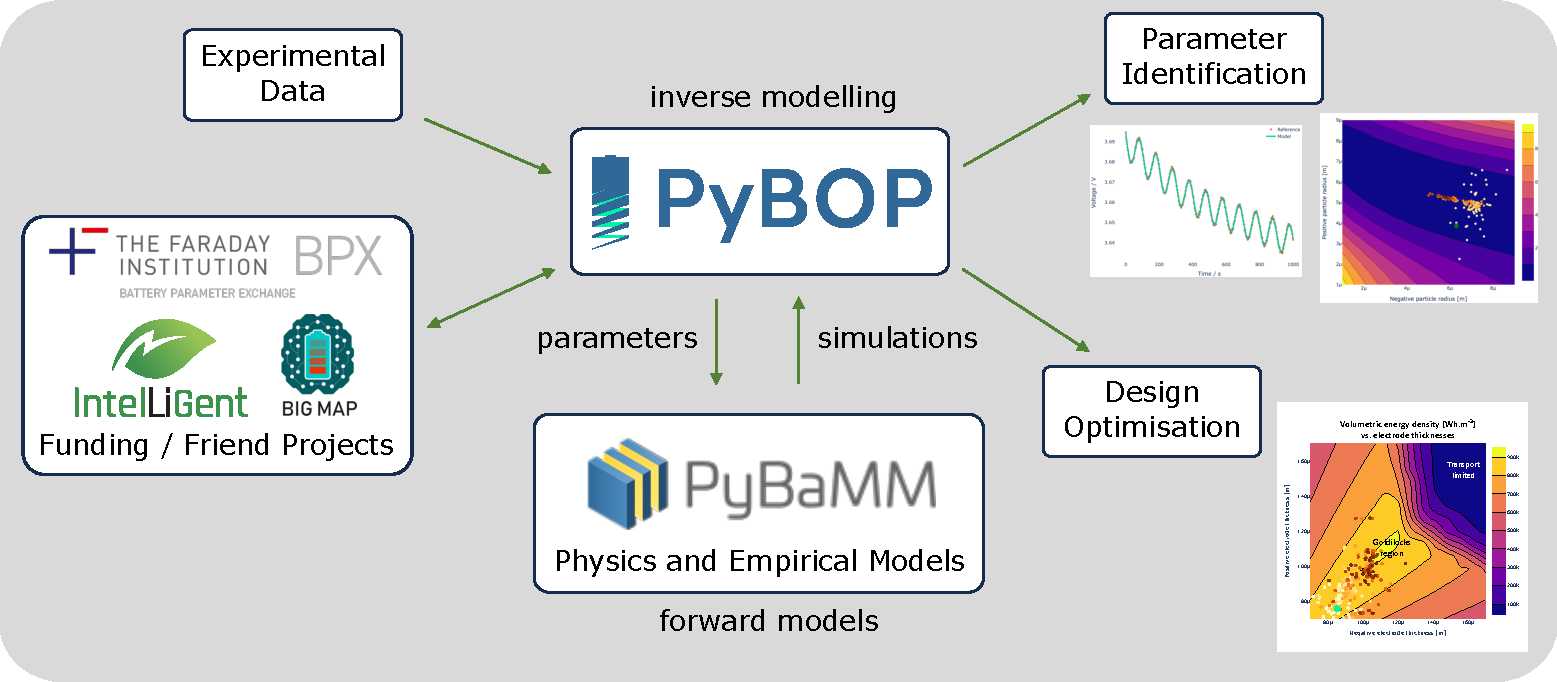
\includegraphics[height=0.42\textwidth]{Images/Diagrams/PyBOP-high-level.pdf}
        \label{fig:project_map}
    \end{figure}
\end{frame}

\section{Updates}

\begin{frame}[plain]
    \centering
    \begin{beamercolorbox}[sep=8pt,center,shadow=true,rounded=true]{title}
    \usebeamerfont{title}{Latest release}\par%
    \color{oxfordblue}\noindent\rule{10cm}{1pt} \\
    \LARGE{\faCloudUpload} \\
    \vspace{6mm} \normalsize
    Aiming for a new release every 3 months. \\
    \href{https://pypi.org/project/pybop/}{https://pypi.org/project/pybop/} \\
    \vspace{6mm}
    The Changelog is updated with new \textbf{features},  \textbf{bug fixes} and \textbf{breaking changes}. \\
    \href{https://github.com/pybop-team/PyBOP/blob/develop/CHANGELOG.md}{https://github.com/pybop-team/PyBOP/blob/develop/CHANGELOG.md}
    \end{beamercolorbox}
\end{frame}


\section{Discussion}

\begin{frame}[plain]
    \centering
    \begin{beamercolorbox}[sep=8pt,center,shadow=true,rounded=true]{title}
    \usebeamerfont{title}{Discussion of open issues}\par%
    \color{oxfordblue}\noindent\rule{10cm}{1pt} \\
    \LARGE{\faUserPlus} \LARGE{\faBug} \\
    \normalsize
    \begin{flushleft}
        Kick-off questions:
    \end{flushleft}
    \begin{itemize}
        \item What issue are you working on/would you like to work on?
        \item Do you have any blockers?
    \end{itemize}
    \vspace{6mm} \normalsize
    Open issues: \href{https://github.com/pybop-team/PyBOP/issues}{https://github.com/pybop-team/PyBOP/issues} \\
    Project board: \href{https://github.com/orgs/pybop-team/projects/}{https://github.com/orgs/pybop-team/projects/}
    \end{beamercolorbox}
\end{frame}

\begin{frame}[plain]
    \centering
    \begin{beamercolorbox}[sep=8pt,center,shadow=true,rounded=true]{title}
    \usebeamerfont{title}{Triage new issues}\par%
    \color{oxfordblue}\noindent\rule{10cm}{1pt} \\
    \end{beamercolorbox}
\end{frame}

\begin{frame}[plain]
    \centering
    \begin{beamercolorbox}[sep=8pt,center,shadow=true,rounded=true]{title}
    \usebeamerfont{title}{Other open items?}\par%
    \color{oxfordblue}\noindent\rule{10cm}{1pt} \\
    \end{beamercolorbox}
\end{frame}

%%%%%%%%%%%%%%%%%%%%%%
%%%% INTRODUCTION %%%%
%%%%%%%%%%%%%%%%%%%%%%

{
\usebackgroundtemplate{
\includegraphics[width=\paperwidth]{Theme/blue_background.png}}%
\begin{frame}[plain]
    \centering
    \begin{beamercolorbox}[sep=8pt,center,shadow=true,rounded=true]{title}
    {\color{white}\usebeamerfont{title}{End of meeting}\par}%
    \color{white}\noindent\rule{10cm}{1pt} \\
    {\color{white}\usebeamerfont{title}{Below: \\
    1. Introductory slides \\
    2. Feature highlights }\par}%
    \end{beamercolorbox}
\end{frame}
}

\section{Introduction}
\begin{frame}[plain]
    \centering
    \begin{beamercolorbox}[sep=8pt,center,shadow=true,rounded=true]{title}
    \usebeamerfont{title}\insertsectionhead\par%
    \color{oxfordblue}\noindent\rule{10cm}{1pt} \\
    \LARGE{\faBatteryThreeQuarters} \\
    \end{beamercolorbox}
    \vspace{6mm} \normalsize
    \begin{flushleft}
        With thanks to:
    \end{flushleft}
    \begin{itemize}
        \item the PyBaMM developers \href{https://github.com/pybop-team/PyBOP}{
\includegraphics[height=1.2em]{Theme/Logos/PyBaMM_logo.png}}
        \item the PINTS developers \href{https://github.com/pints-team/pints}{\faGithub}
    \end{itemize}
\end{frame}


\begin{frame}{Aims}
    \vspace{-6mm}
    \begin{figure}
        \centering
        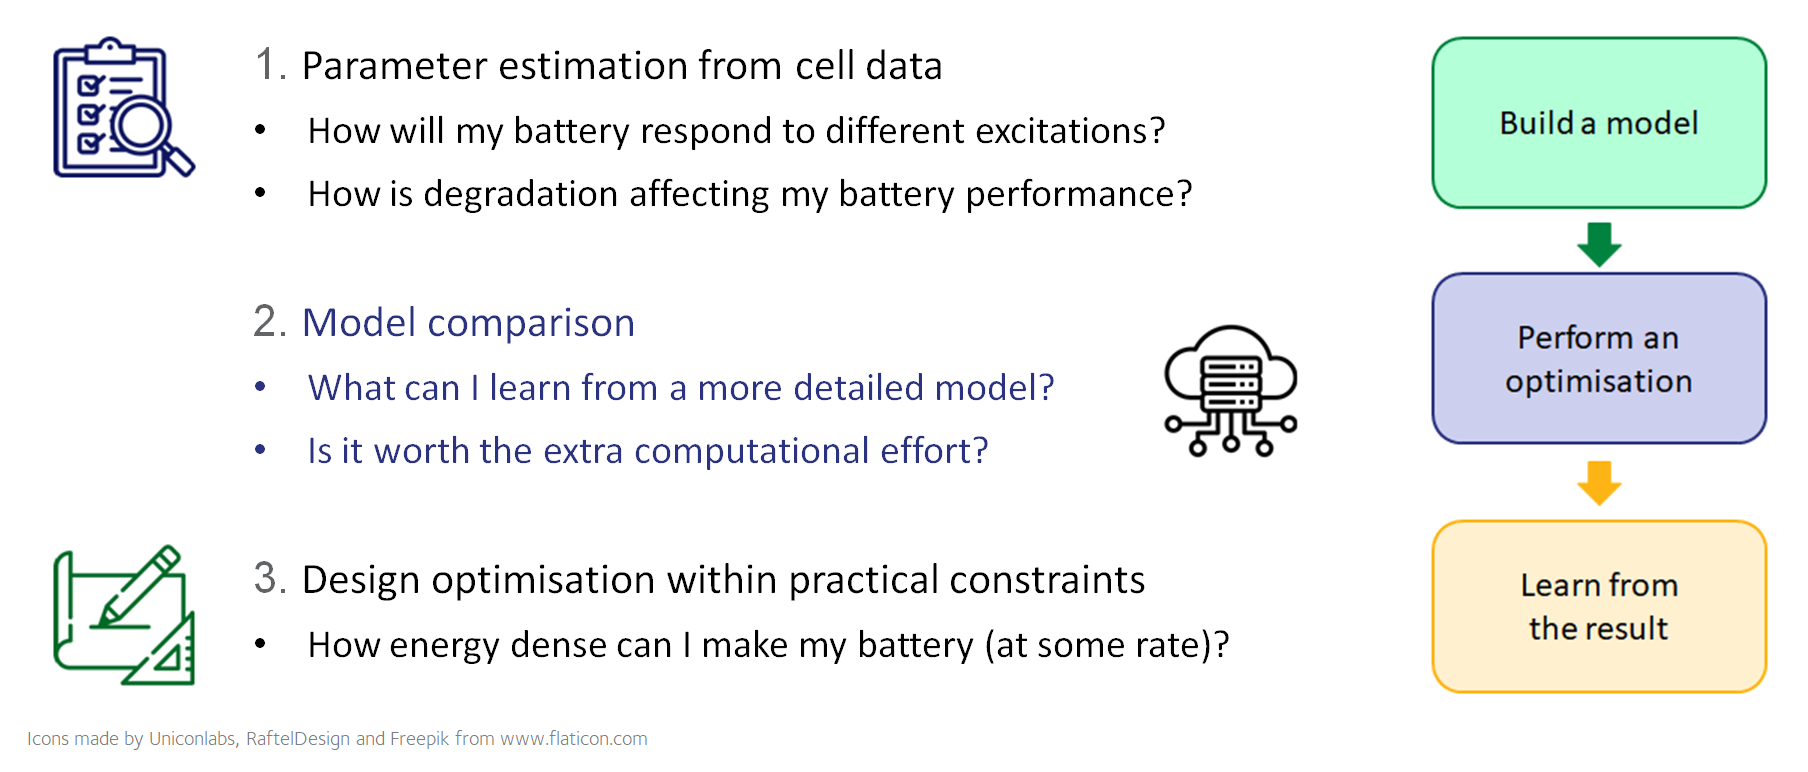
\includegraphics[width=\textwidth]{Images/Diagrams/ProblemTypes.png}
    \end{figure}
\end{frame}

\begin{frame}{Architecture}
    \vspace{-6mm}
    \begin{figure}
        \centering
        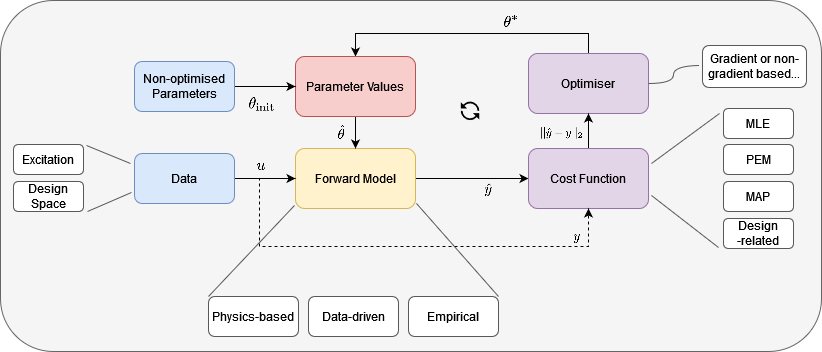
\includegraphics[width=0.9\textwidth]{Images/Diagrams/pybop_architecture.png}
        % \caption{Caption}
        \label{fig:architecture}
    \end{figure}
\end{frame}

\begin{frame}{Python objects}
    \vspace{-6mm}
    \begin{figure}
        \centering
        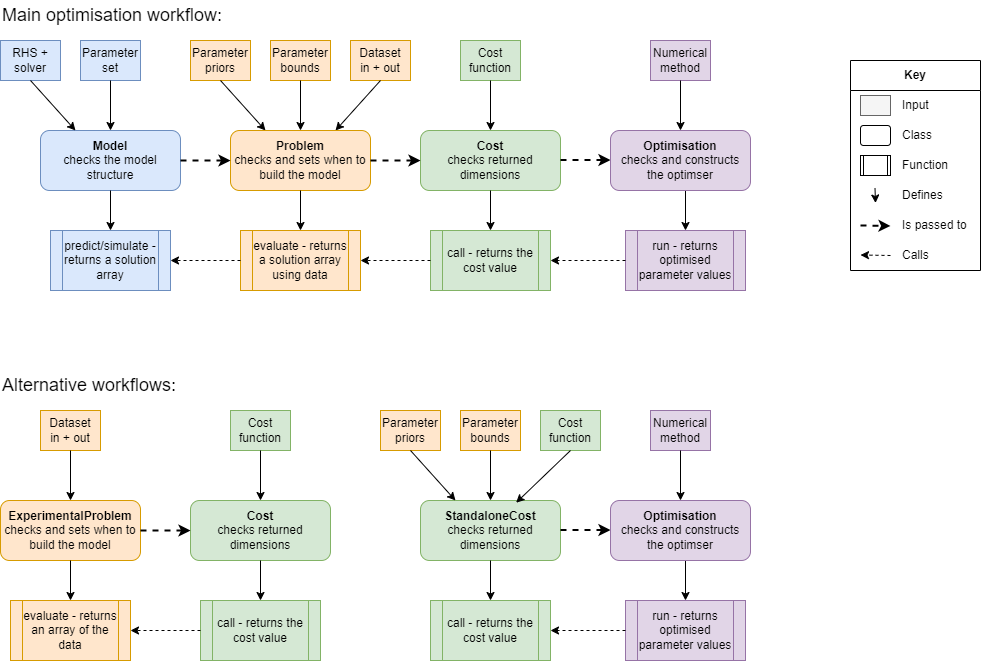
\includegraphics[width=0.95\textwidth, trim={0 10cm 0 0},clip]{Images/Diagrams/pybop_objects.png}
        % \caption{Caption}
        \label{fig:objects}
    \end{figure}
\end{frame}


\section{Demo/examples}
\begin{frame}[plain]
    \centering
    \begin{beamercolorbox}[sep=8pt,center,shadow=true,rounded=true]{title}
    \usebeamerfont{title}\insertsectionhead\par%
    \color{oxfordblue}\noindent\rule{10cm}{1pt} \\
    \LARGE{\faFileCodeO} \\
    \normalsize
    \begin{itemize}
        \item Parameterisation
        \item Design optimisation
    \end{itemize}
    \end{beamercolorbox}
\end{frame}

\subsection{Parameterisation example}
\begin{frame}[fragile,t]{Parameterisation}
    \vspace{-0.5cm}
    \begin{block}{1. Define a model (PyBaMM's SPM) and fitting parameters}
    \begin{lstlisting}[firstnumber=1, xleftmargin=10pt]
import pybop
import numpy as np

# Define model
parameter_set = pybop.ParameterSet.pybamm("Chen2020")
model = pybop.lithium_ion.SPM(parameter_set=parameter_set)

# Fitting parameters
parameters = pybop.Parameters(
    pybop.Parameter(
        "Negative particle radius [m]",
        prior=pybop.Gaussian(6e-06, 0.1e-6),
        bounds=[1e-6, 9e-6],
    ),
    pybop.Parameter(
        "Positive particle radius [m]",
        prior=pybop.Gaussian(4.5e-06, 0.1e-6),
        bounds=[1e-6, 9e-6],
    ),
)
    \end{lstlisting}
    \end{block}
\end{frame}

\subsection{Parameterisation example}
\begin{frame}[fragile,t]{Parameterisation}
    \vspace{-0.5cm}
    \begin{block}{2. Generate synthetic data and define problem, cost and optimisation}
    \begin{lstlisting}[firstnumber=1, xleftmargin=10pt]
# Generate data
sigma = 0.001
t_eval = np.arange(0, 900, 3)
values = model.predict(t_eval=t_eval)
corrupt_values = values["Voltage [V]"].data + np.random.normal(0, sigma, len(t_eval))

# Form dataset
dataset = pybop.Dataset(
    {
        "Time [s]": t_eval,
        "Current function [A]": values["Current [A]"].data,
        "Voltage [V]": corrupt_values,
    }
)

# Generate problem, cost function, and optimisation class
problem = pybop.FittingProblem(model, parameters, dataset)
cost = pybop.SumSquaredError(problem)
optim = pybop.CMAES(cost, max_iterations=100)
    \end{lstlisting}
    \end{block}
\end{frame}

\subsection{Parameterisation example}
\begin{frame}[fragile,t]{Parameterisation}
    \vspace{-1.5cm}
    \begin{block}{3. Run the optimisation and plot the results}
    \begin{lstlisting}[firstnumber=1, xleftmargin=10pt]
# Run the optimisation
x, final_cost = optim.run()
print("True parameters:", parameters.true_value())
print("Estimated parameters:", x)

# Plot the timeseries output
pybop.quick_plot(problem, problem_inputs=x, title="Optimised Comparison")

# Plot convergence and parameter traces
pybop.plot_convergence(optim)

# Plot the parameter traces
pybop.plot_parameters(optim)

# Plot the cost landscape with optimisation path
pybop.plot2d(optim, steps=15)
    \end{lstlisting}
    \end{block}
\end{frame}

\begin{frame}{Parameterisation results}
    \vspace{-6mm}
    \begin{figure}
        \centering
        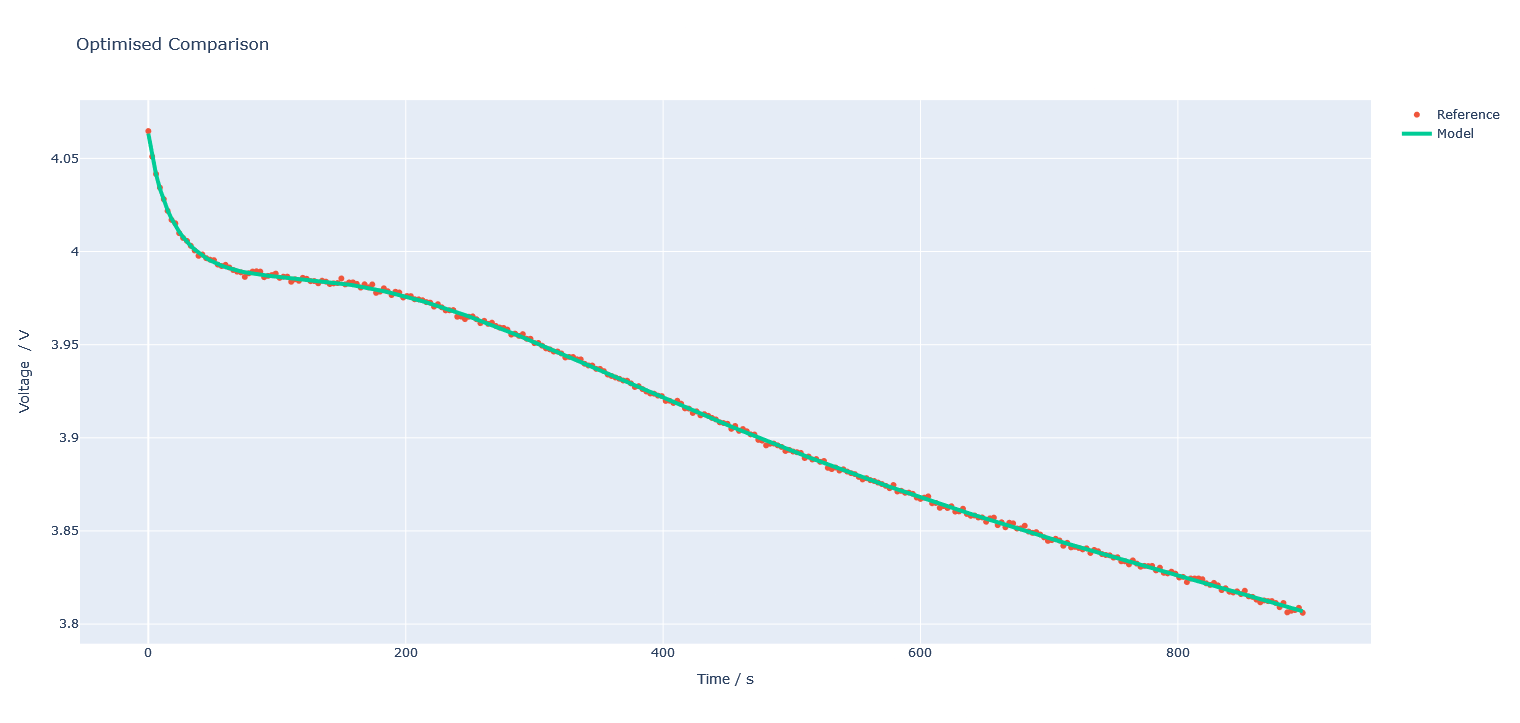
\includegraphics[width=0.4\textwidth, trim={0 0 0 0},clip]{Images/Examples/CMAES_quick_plot.png}
        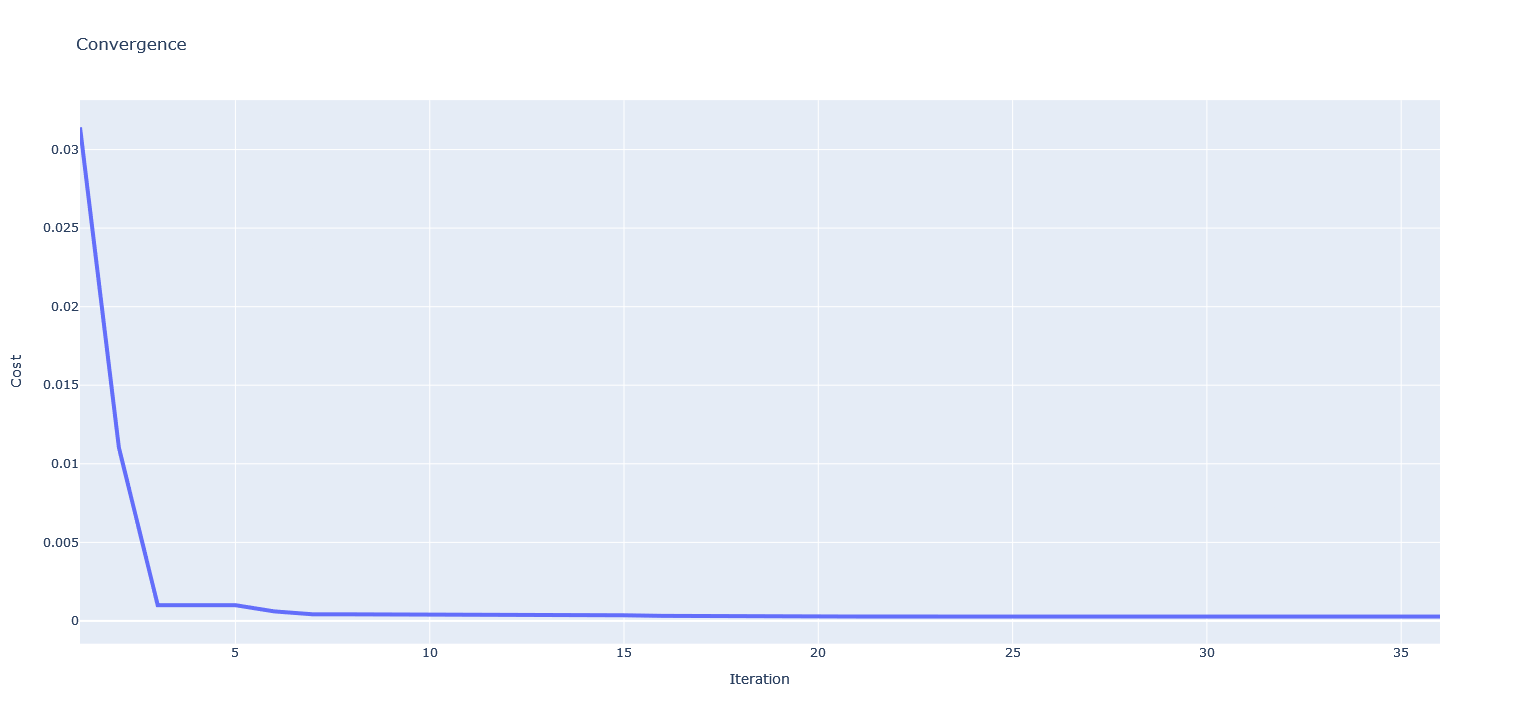
\includegraphics[width=0.4\textwidth, trim={0 0 0 0},clip]{Images/Examples/CMAES_convergence.png} \\
        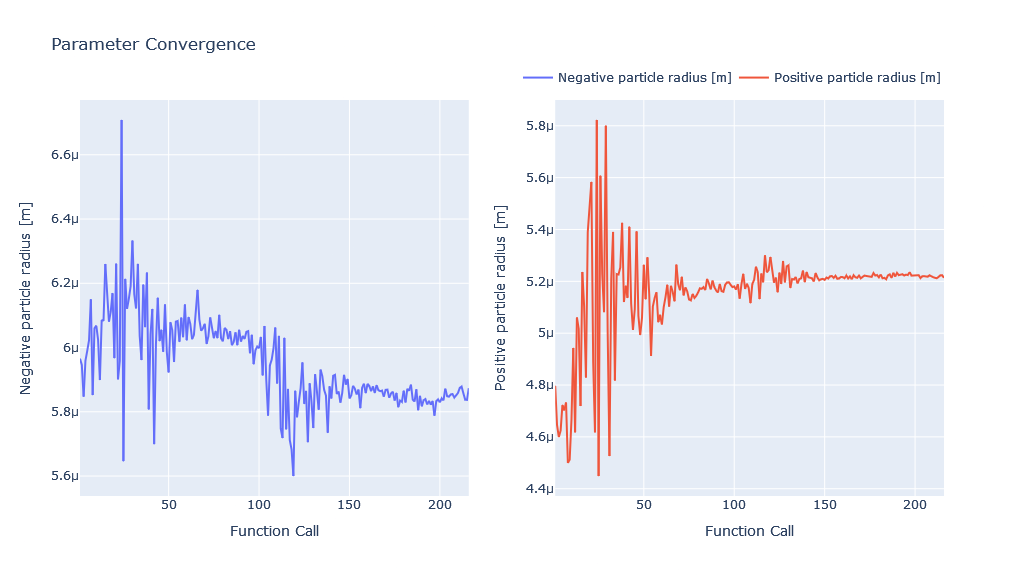
\includegraphics[width=0.5\textwidth, trim={0 0 0 0},clip]{Images/Examples/CMAES_parameters.png}
        \hspace{1cm}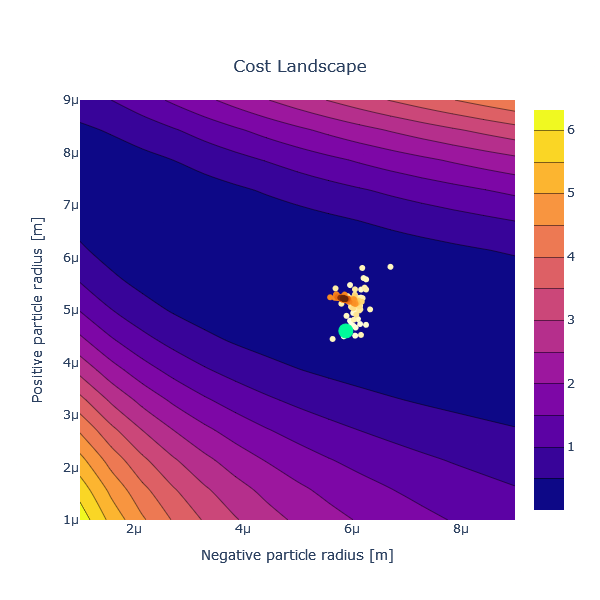
\includegraphics[width=0.29\textwidth, trim={0 0 0 0},clip]{Images/Examples/CMAES_cost_trace.png}
        \hspace{1cm}
        \label{fig:parameterisation}
    \end{figure}
\end{frame}

\subsection{Design optimisation example}
\begin{frame}[fragile,t]{Design optimisation}
    \vspace{-1.5cm}
    \begin{block}{1. Define a model (PyBaMM's SPMe) and design parameters}
    \begin{lstlisting}[firstnumber=1, xleftmargin=10pt]
import pybop
import numpy as np

# Define parameter set and model
parameter_set = pybop.ParameterSet.pybamm("Chen2020", formation_concentrations=True)
model = pybop.lithium_ion.SPMe(parameter_set=parameter_set)

# Fitting parameters
parameters = pybop.Parameters(
    pybop.Parameter(
        "Positive electrode thickness [m]",
        prior=pybop.Gaussian(7.56e-05, 0.05e-05),
        bounds=[65e-06, 10e-05],
    ),
    pybop.Parameter(
        "Positive particle radius [m]",
        prior=pybop.Gaussian(5.22e-06, 0.05e-06),
        bounds=[2e-06, 9e-06],
    ),
)
    \end{lstlisting}
    \end{block}
\end{frame}

\begin{frame}[fragile,t]{Design optimisation}
    \vspace{-1cm}
    \begin{block}{2. Set the target experiment and define problem, cost and optimisation}
    \begin{lstlisting}[firstnumber=1, xleftmargin=10pt]
# Define test protocol
experiment = pybop.Experiment(
    ["Discharge at 1C until 2.5 V (5 seconds period)"],
)
init_soc = 1  # start from full charge
signal = ["Voltage [V]", "Current [A]"]

# Generate problem
problem = pybop.DesignProblem(
    model, parameters, experiment, signal=signal, init_soc=init_soc
)

# Generate cost function and optimisation class:
cost = pybop.GravimetricEnergyDensity(problem, update_capacity=True)
optim = pybop.PSO(
    cost, verbose=True, allow_infeasible_solutions=False, max_iterations=15
)
    \end{lstlisting}
    \end{block}
\end{frame}

\begin{frame}[fragile,t]{Design optimisation}
    \vspace{-2cm}
    \begin{block}{3. Run the optimisation and plot the results}
    \begin{lstlisting}[firstnumber=1, xleftmargin=10pt]
# Run optimisation
x, final_cost = optim.run()
print("Estimated parameters:", x)
print(f"Initial gravimetric energy density: {cost(optim.x0):.2f} Wh.kg-1")
print(f"Optimised gravimetric energy density: {final_cost:.2f} Wh.kg-1")

# Plot the timeseries output
if cost.update_capacity:
    problem._model.approximate_capacity(x)
pybop.quick_plot(problem, problem_inputs=x, title="Optimised Comparison")

# Plot the cost landscape with optimisation path
pybop.plot2d(optim, steps=10)
    \end{lstlisting}
    \end{block}
\end{frame}

\begin{frame}[fragile,t]{Design optimisation}
    \vspace{-6mm}
    \begin{block}{Output}
    \begin{lstlisting}[firstnumber=1, xleftmargin=10pt]
Estimated parameters: [6.51159429e-05 2.32340723e-06]
Initial gravimetric energy density: 386.31 Wh.kg-1
Optimised gravimetric energy density: 410.78 Wh.kg-1
    \end{lstlisting}
    \end{block}
    Results
    \vspace{-3mm}
    \begin{figure}
        \centering
        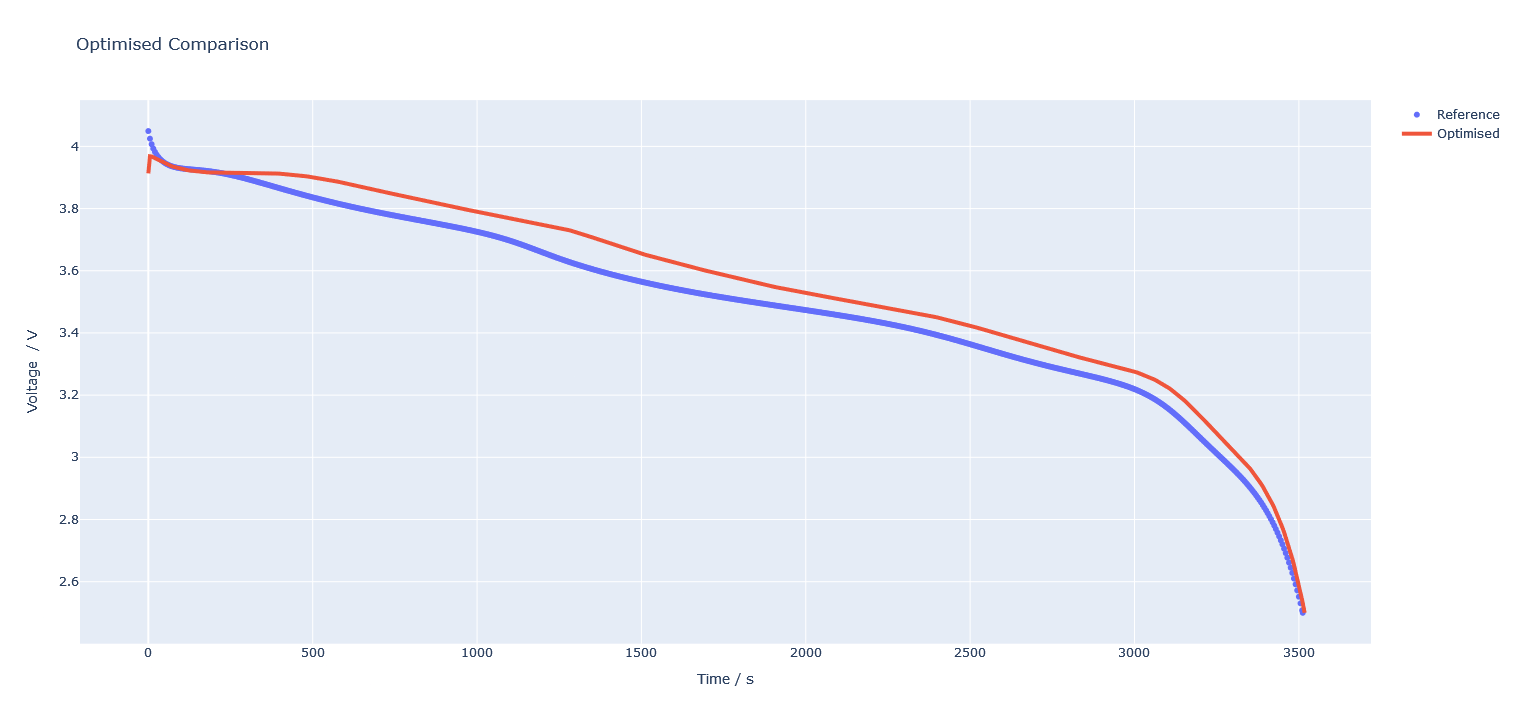
\includegraphics[width=0.59\textwidth, trim={0 0 0 0},clip]{Images/Examples/MaxEnergy_quick_plot.png}
        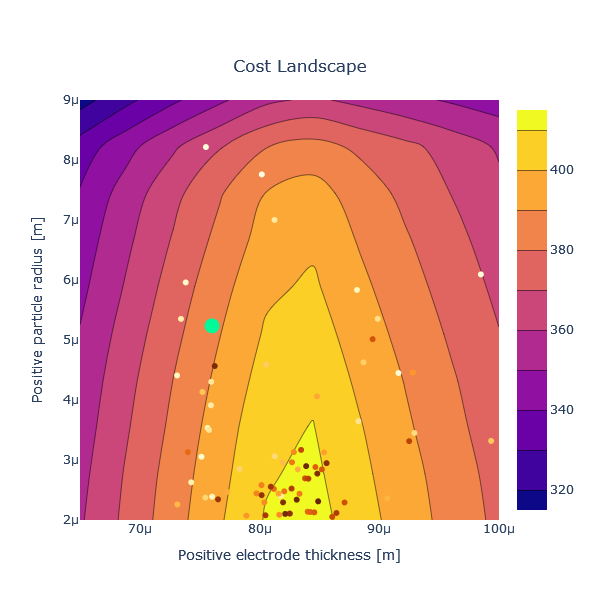
\includegraphics[width=0.29\textwidth, trim={0 0 0 0},clip]{Images/Examples/MaxEnergy_cost_trace.png} \\
        \label{fig:design_optimisation}
    \end{figure}
\end{frame}


\section{Choice of optimisers}
\begin{frame}[plain]
    \centering
    \begin{beamercolorbox}[sep=8pt,center,shadow=true,rounded=true]{title}
    \usebeamerfont{title}\insertsectionhead\par%
    \color{oxfordblue}\noindent\rule{10cm}{1pt} \\
    \LARGE{\faBalanceScale} \\
    \end{beamercolorbox}
\end{frame}

\subsection{Gradient-based optimisers}
\begin{frame}{Gradient-based}
    \vspace{-6mm}
    \begin{table}[]
        \centering
        \footnotesize
    \begin{tabularx}{0.86\textwidth}{*{3}{Y}}
         Gradient descent &
         Adaptive moment (AdamW) &
         Resilient backpropagation (IRPropMin)
    \end{tabularx}
    \end{table}

    \vspace{-6mm}
    \begin{figure}
        \centering
        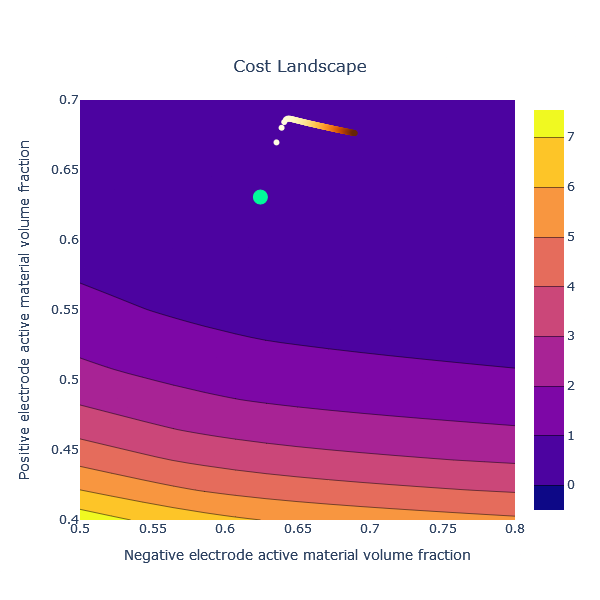
\includegraphics[width=0.24\textwidth]{Images/Optimisers/graddesc_cost.png}
        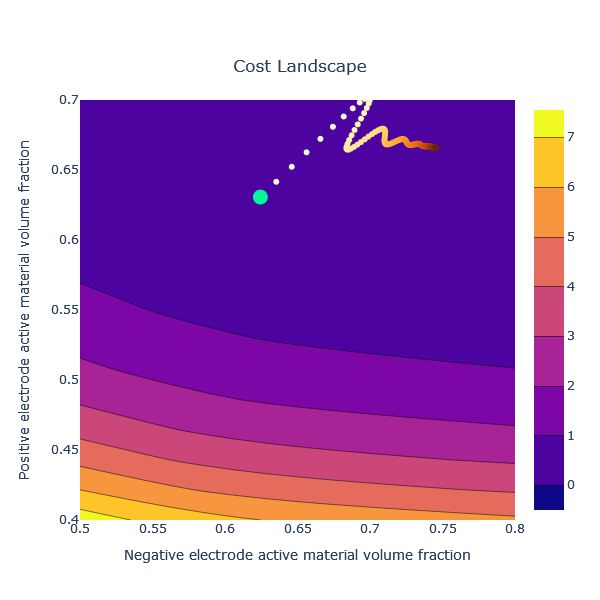
\includegraphics[width=0.24\textwidth]{Images/Optimisers/adamw_cost.png}
        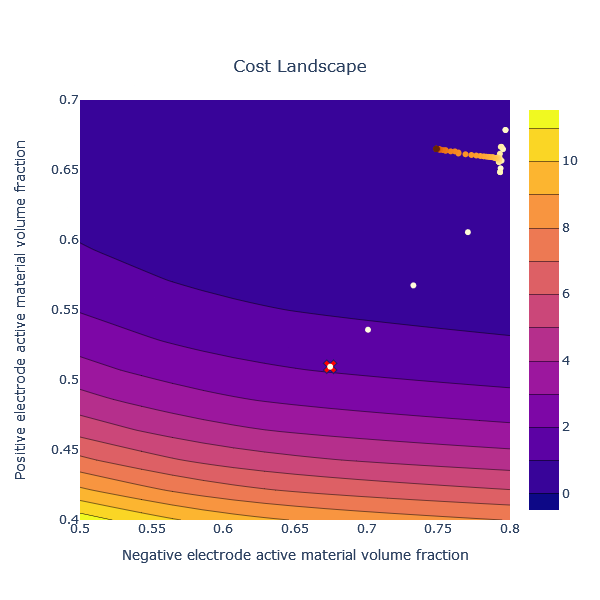
\includegraphics[width=0.24\textwidth]{Images/Optimisers/irpropmin_cost.png} ~~~\\
        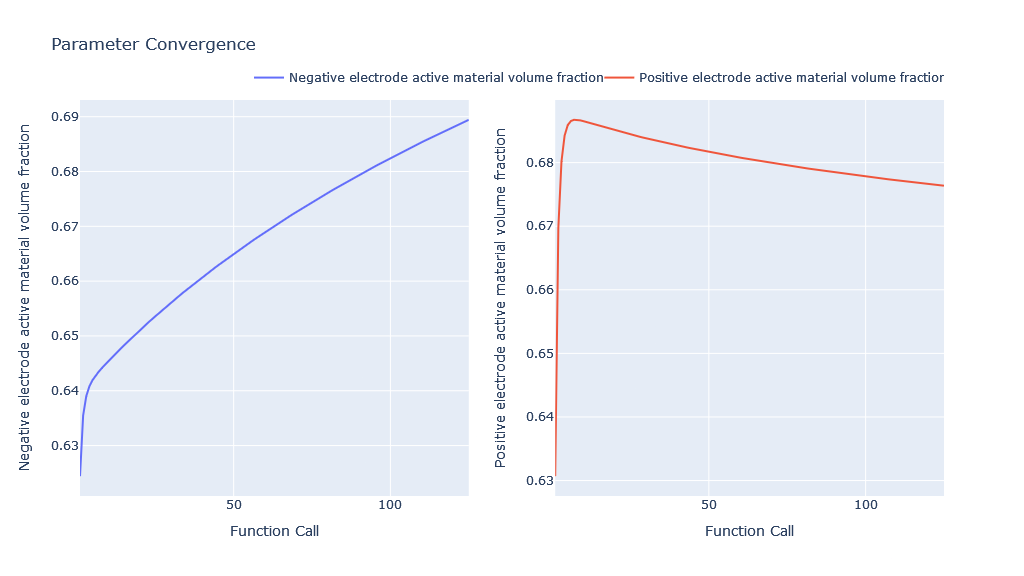
\includegraphics[width=0.24\textwidth]{Images/Optimisers/graddesc_params.png}
        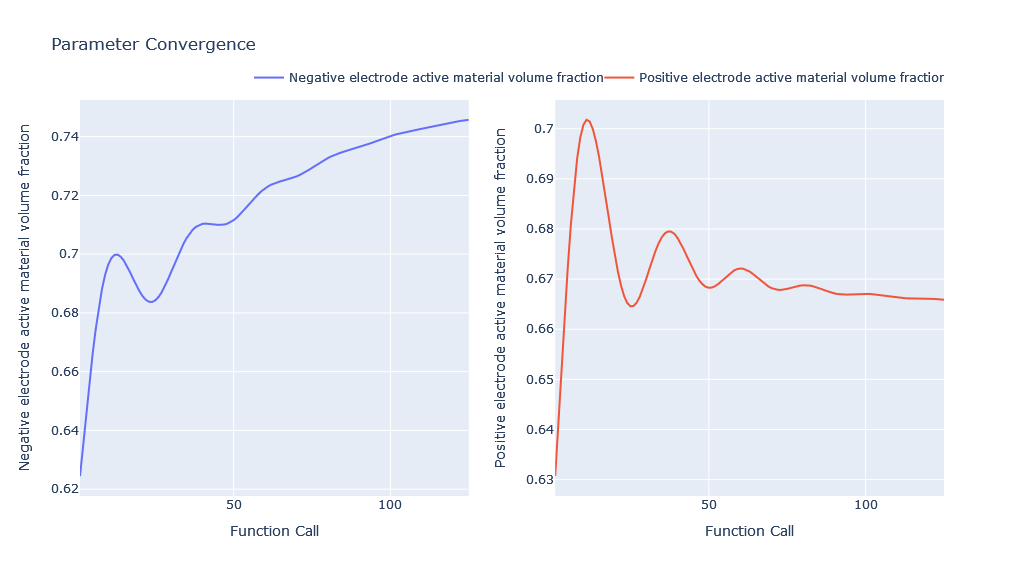
\includegraphics[width=0.24\textwidth]{Images/Optimisers/adamw_params.png}
        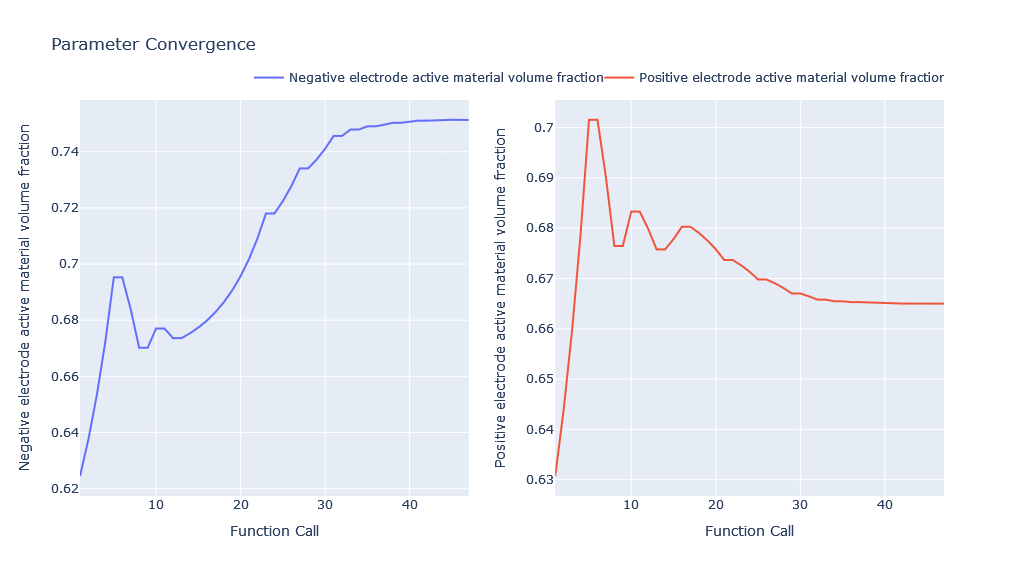
\includegraphics[width=0.24\textwidth]{Images/Optimisers/irpropmin_params.png}
        % \caption{Caption}
        \label{fig:optimisers1}
    \end{figure}
\end{frame}

\subsection{Non-gradient-based optimisers}
\begin{frame}{Evolution strategies}
    \vspace{-5mm}
    \begin{table}[]
        \centering
        \footnotesize
    \begin{tabularx}{0.86\textwidth}{*{3}{Y}}
         Stochastic natural evolution strategy (SNES) &
         Exponential natural evolution strategy (SNES) &
         Covariance matrix adaptation (CMA-ES)
    \end{tabularx}
    \end{table}

    \vspace{-5mm}
    \begin{figure}
        \centering
        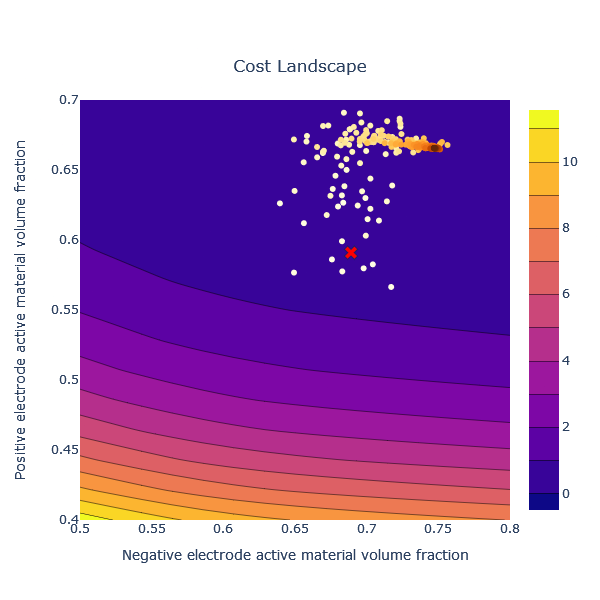
\includegraphics[width=0.24\textwidth]{Images/Optimisers/snes_cost.png}
        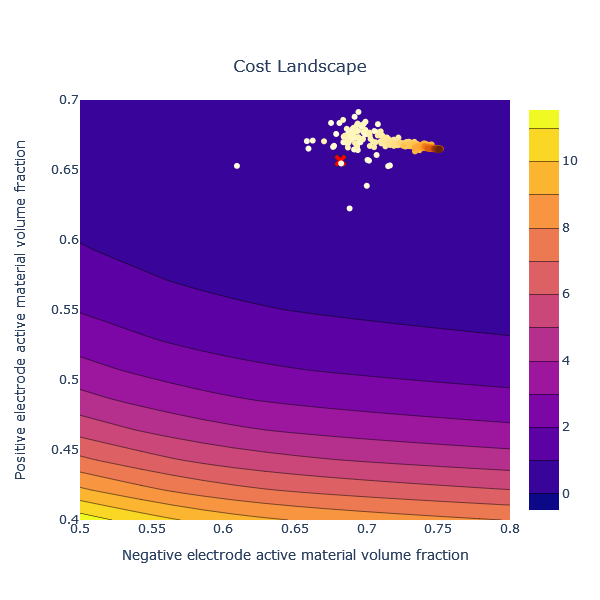
\includegraphics[width=0.24\textwidth]{Images/Optimisers/xnes_cost.png}
        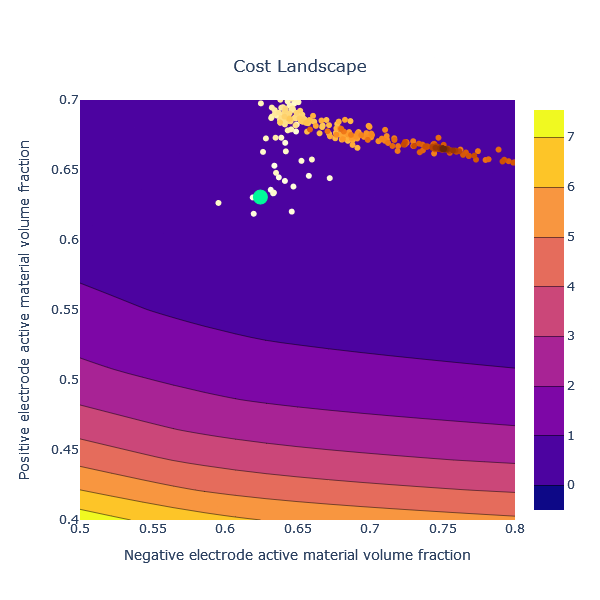
\includegraphics[width=0.24\textwidth]{Images/Optimisers/cmaes_cost.png} ~~~\\
        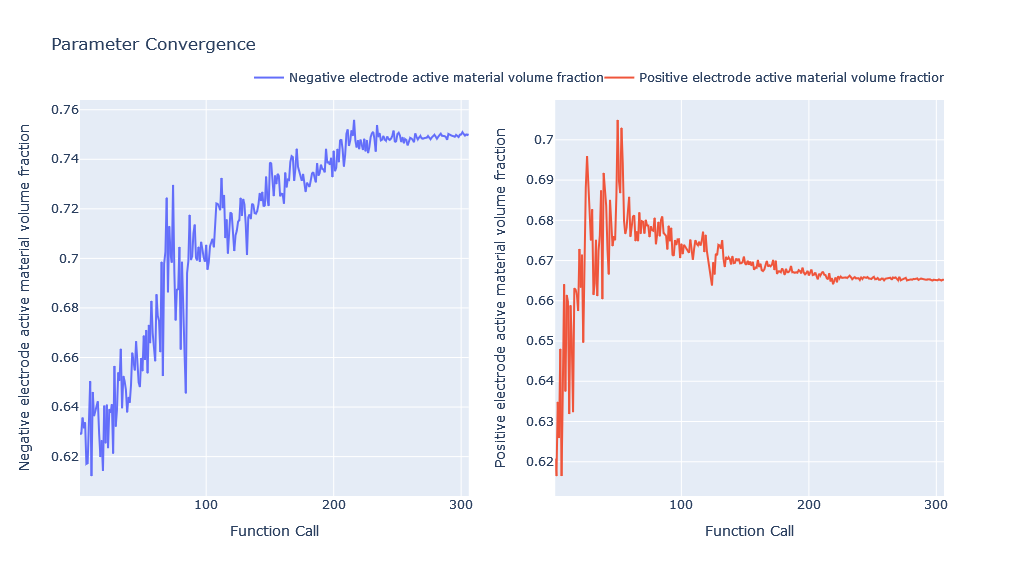
\includegraphics[width=0.24\textwidth]{Images/Optimisers/snes_params.png}
        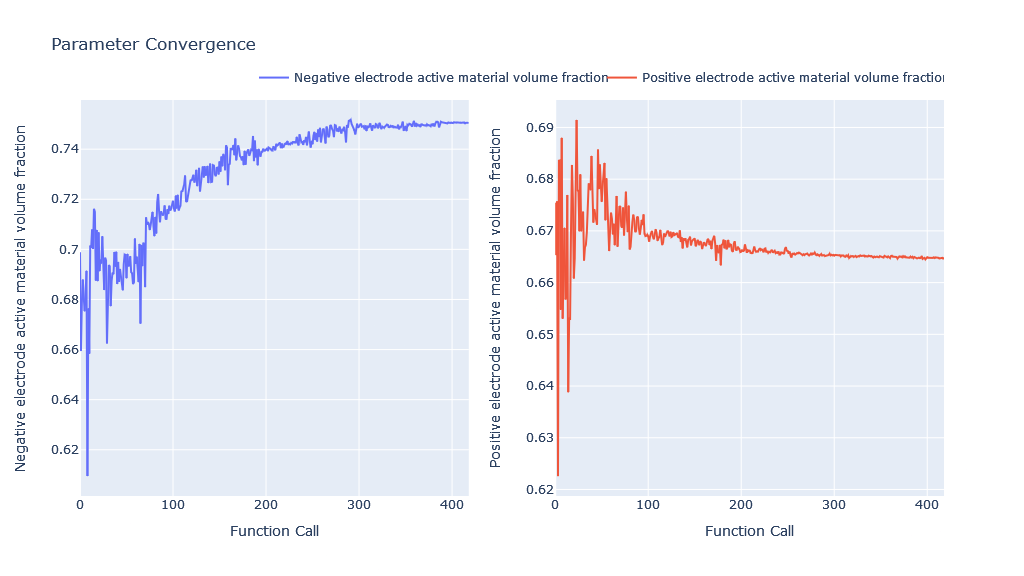
\includegraphics[width=0.24\textwidth]{Images/Optimisers/xnes_params.png}
        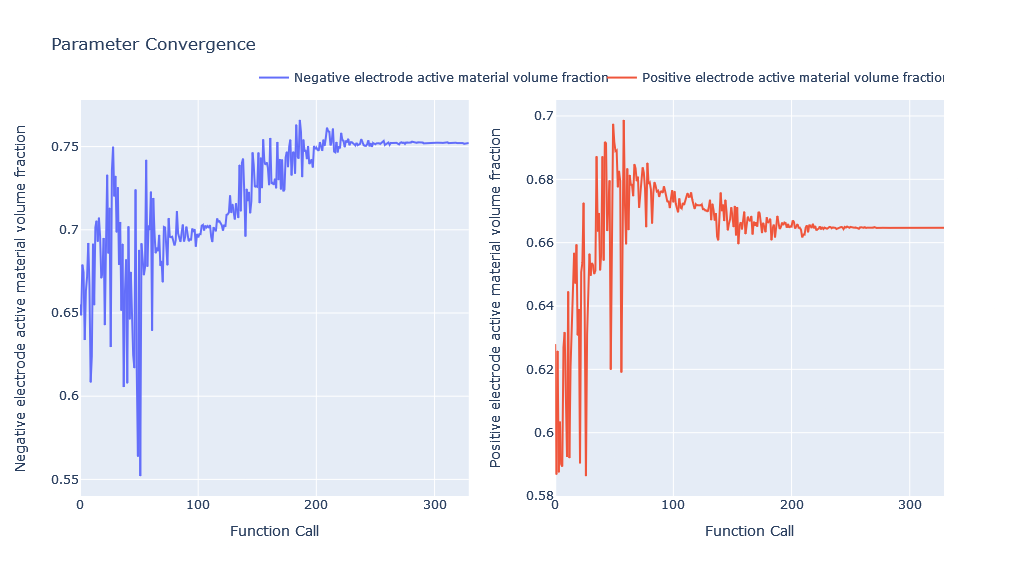
\includegraphics[width=0.24\textwidth]{Images/Optimisers/cmaes_params.png}
        % \caption{Caption}
        \label{fig:optimisers4}
    \end{figure}
\end{frame}

\begin{frame}{Other optimisers}
    \vspace{-6mm}
    \begin{table}[]
        \centering
        \footnotesize
    \begin{tabularx}{\textwidth}{*{4}{Y}}
         Nelder Mead &
         Particle swarm optimisation &
         SciPy differential evolution
    \end{tabularx}
    \end{table}

    \vspace{-6mm}
    \begin{figure}
        \centering
        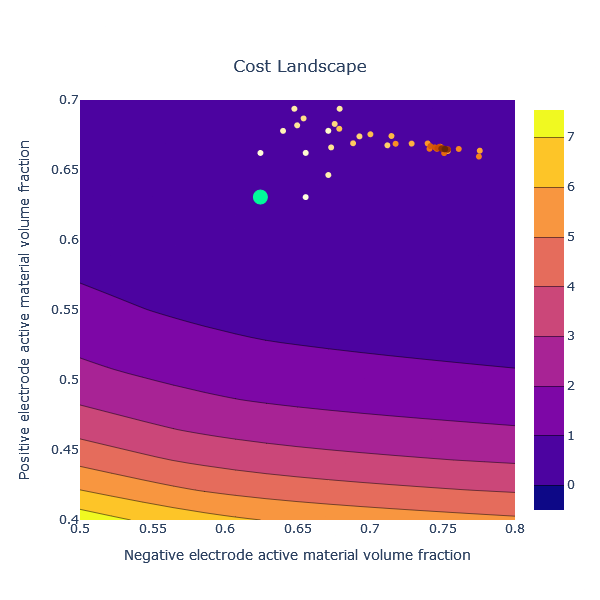
\includegraphics[width=0.24\textwidth]{Images/Optimisers/neldermead_cost.png}
        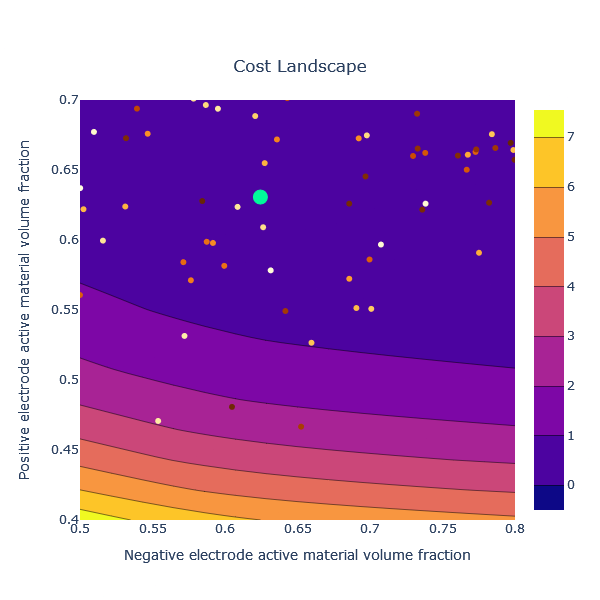
\includegraphics[width=0.24\textwidth]{Images/Optimisers/pso_cost.png}
        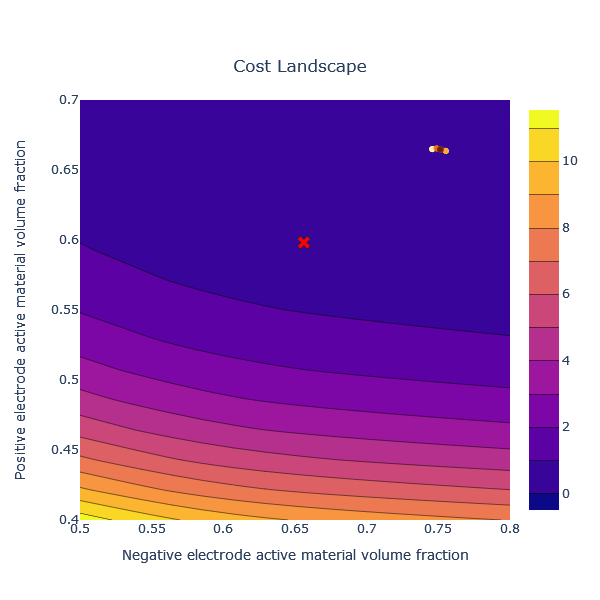
\includegraphics[width=0.24\textwidth]{Images/Optimisers/scipyde_cost.png} ~~~~\\
        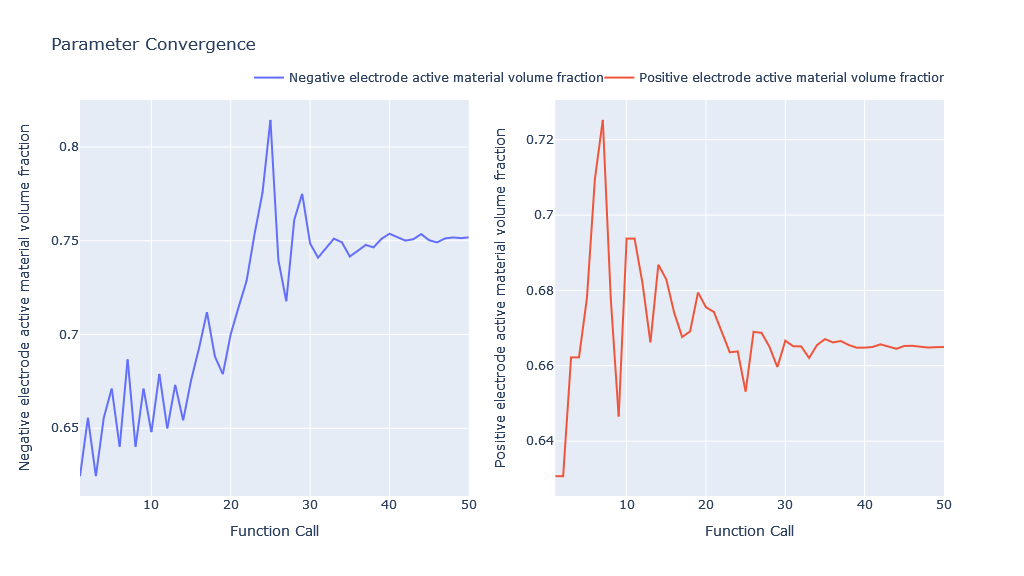
\includegraphics[width=0.24\textwidth]{Images/Optimisers/neldermead_params.png}
        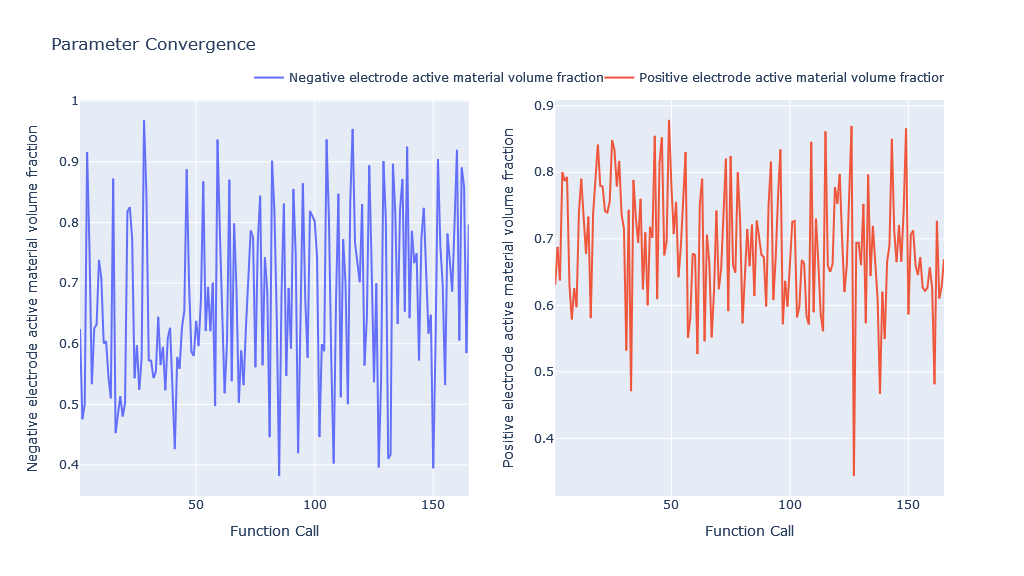
\includegraphics[width=0.24\textwidth]{Images/Optimisers/pso_params.png}
        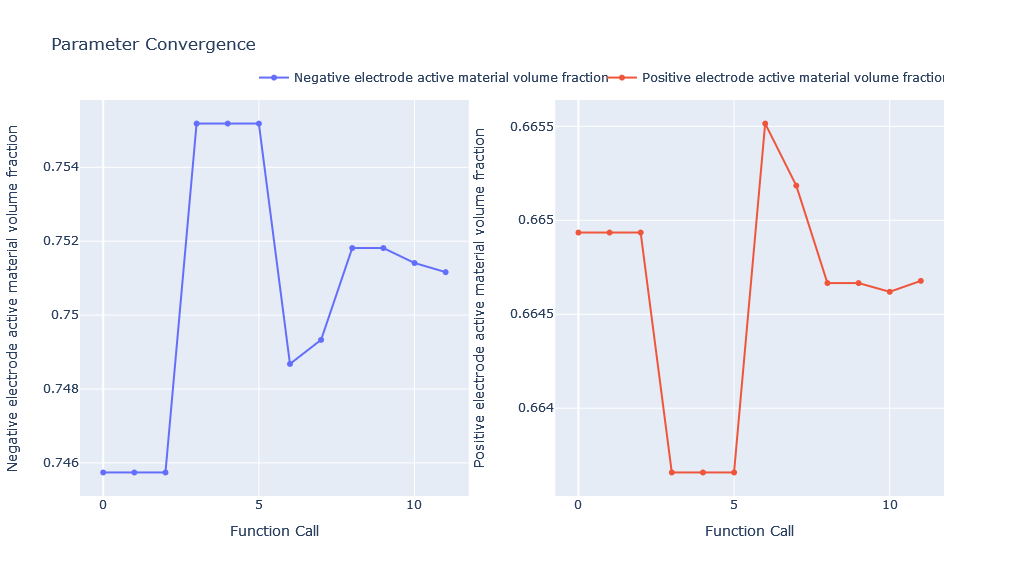
\includegraphics[width=0.24\textwidth]{Images/Optimisers/scipyde_params.png}
        \label{fig:optimisers2}
    \end{figure}
\end{frame}

\begin{frame}{Collaboration}
    \vspace{-6mm}
    \begin{figure}
        \centering
        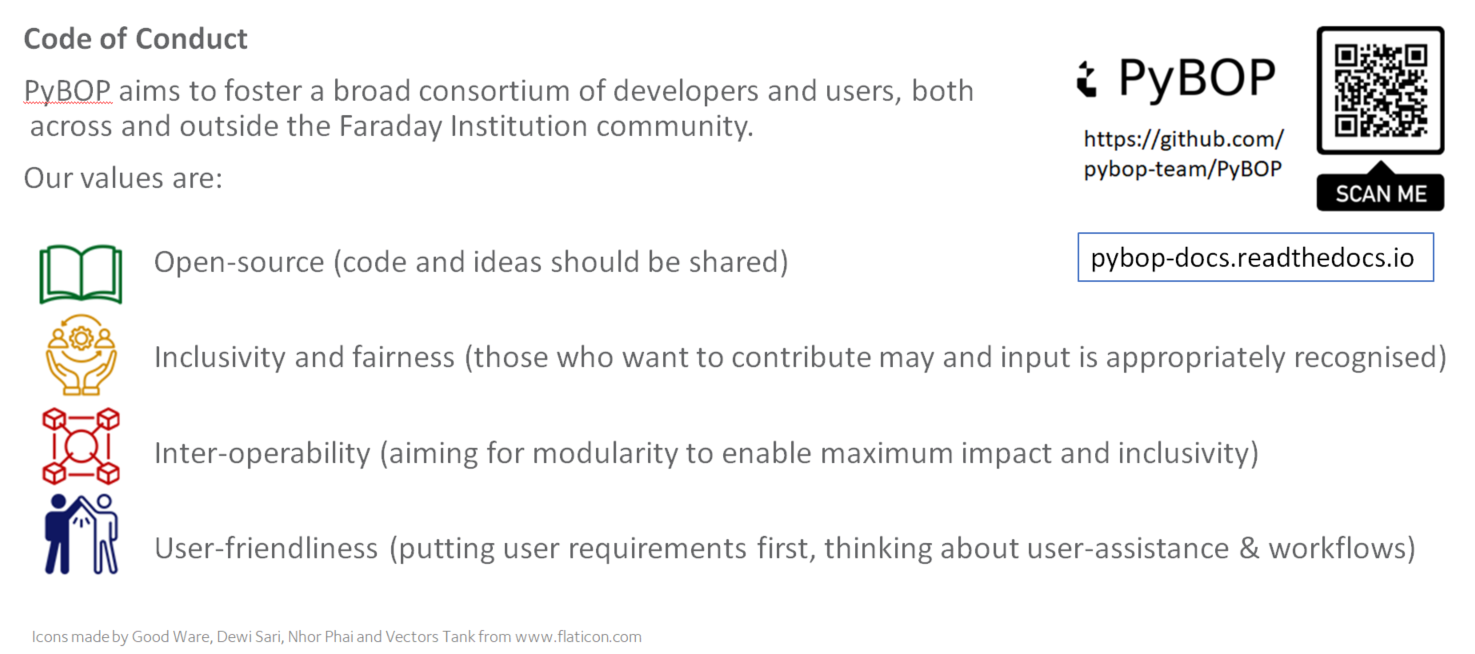
\includegraphics[width=\textwidth]{Images/Code_of_Conduct.png}
    \end{figure}
\end{frame}

\section{Feature highlights}
\begin{frame}[plain]
    \centering
    \begin{beamercolorbox}[sep=8pt,center,shadow=true,rounded=true]{title}
    \usebeamerfont{title}\insertsectionhead\par%
    \color{oxfordblue}\noindent\rule{10cm}{1pt} \\
    \LARGE{\faBatteryThreeQuarters} \\
    \end{beamercolorbox}
\end{frame}

\begin{frame}[fragile,t]{New in v24.9: New costs and samplers}
    \vspace{-6mm}
    \issue{462} - Adds Minkowski and SumofPower cost functions. \\
    \issue{6} - Adds Monte Carlo Sampling classes

    \begin{figure}
        \centering
        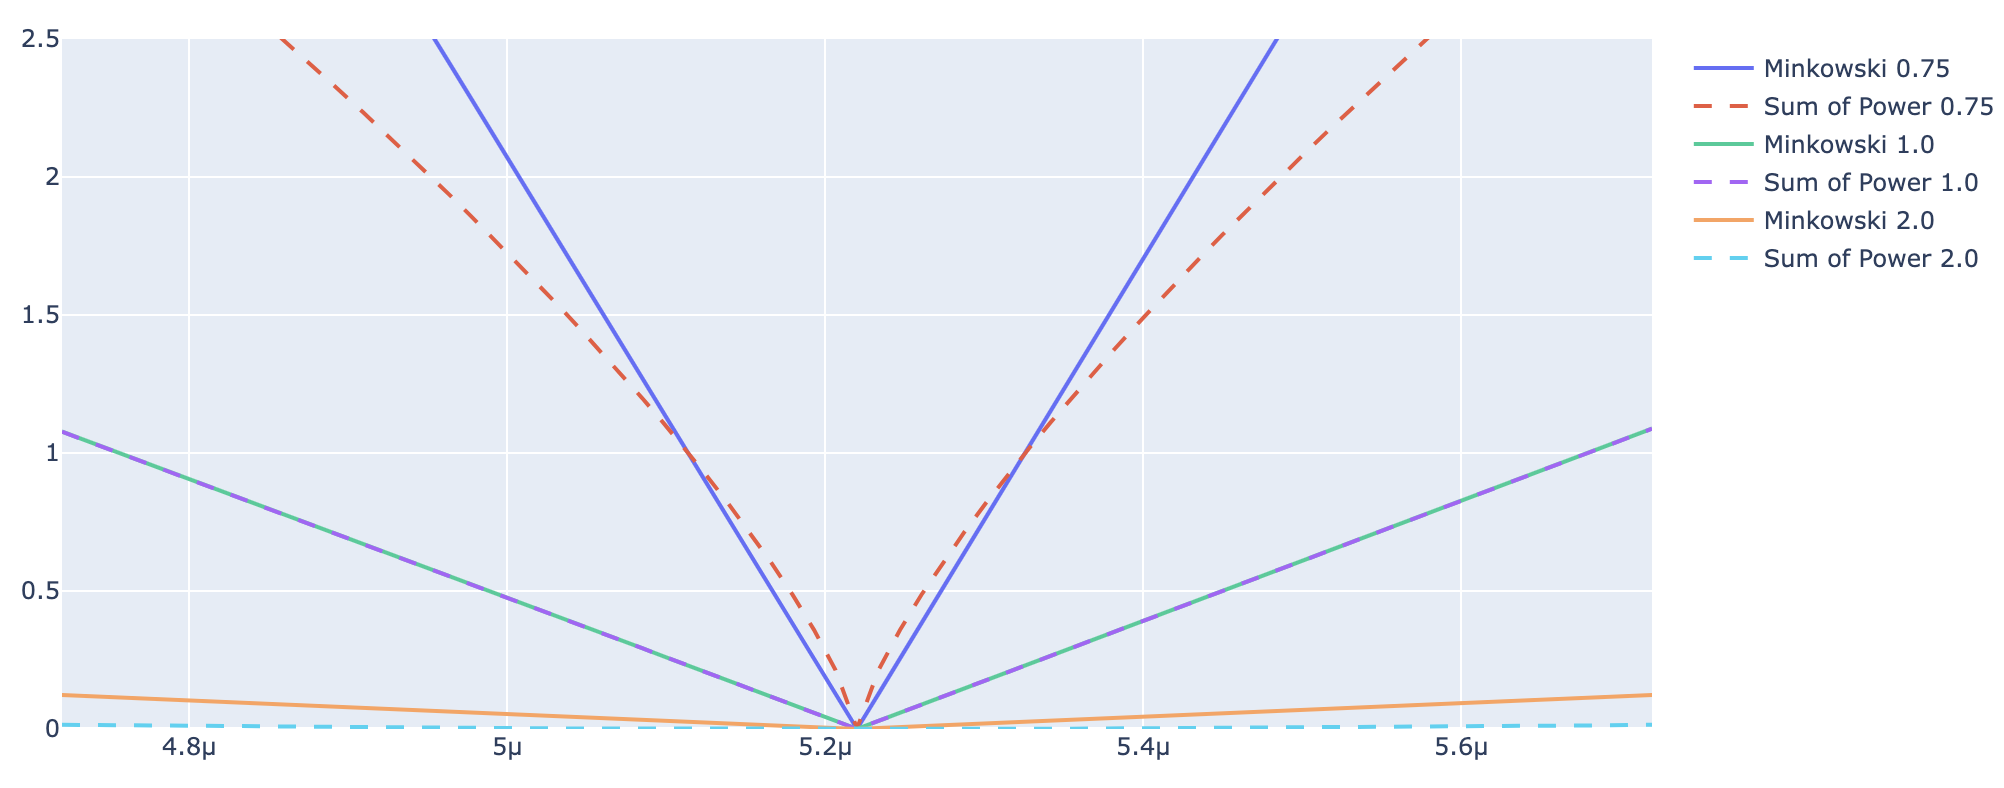
\includegraphics[width=0.5\textwidth]{Images/Highlights/minkowski-sum-of-power.png}
        \hspace{1em}
        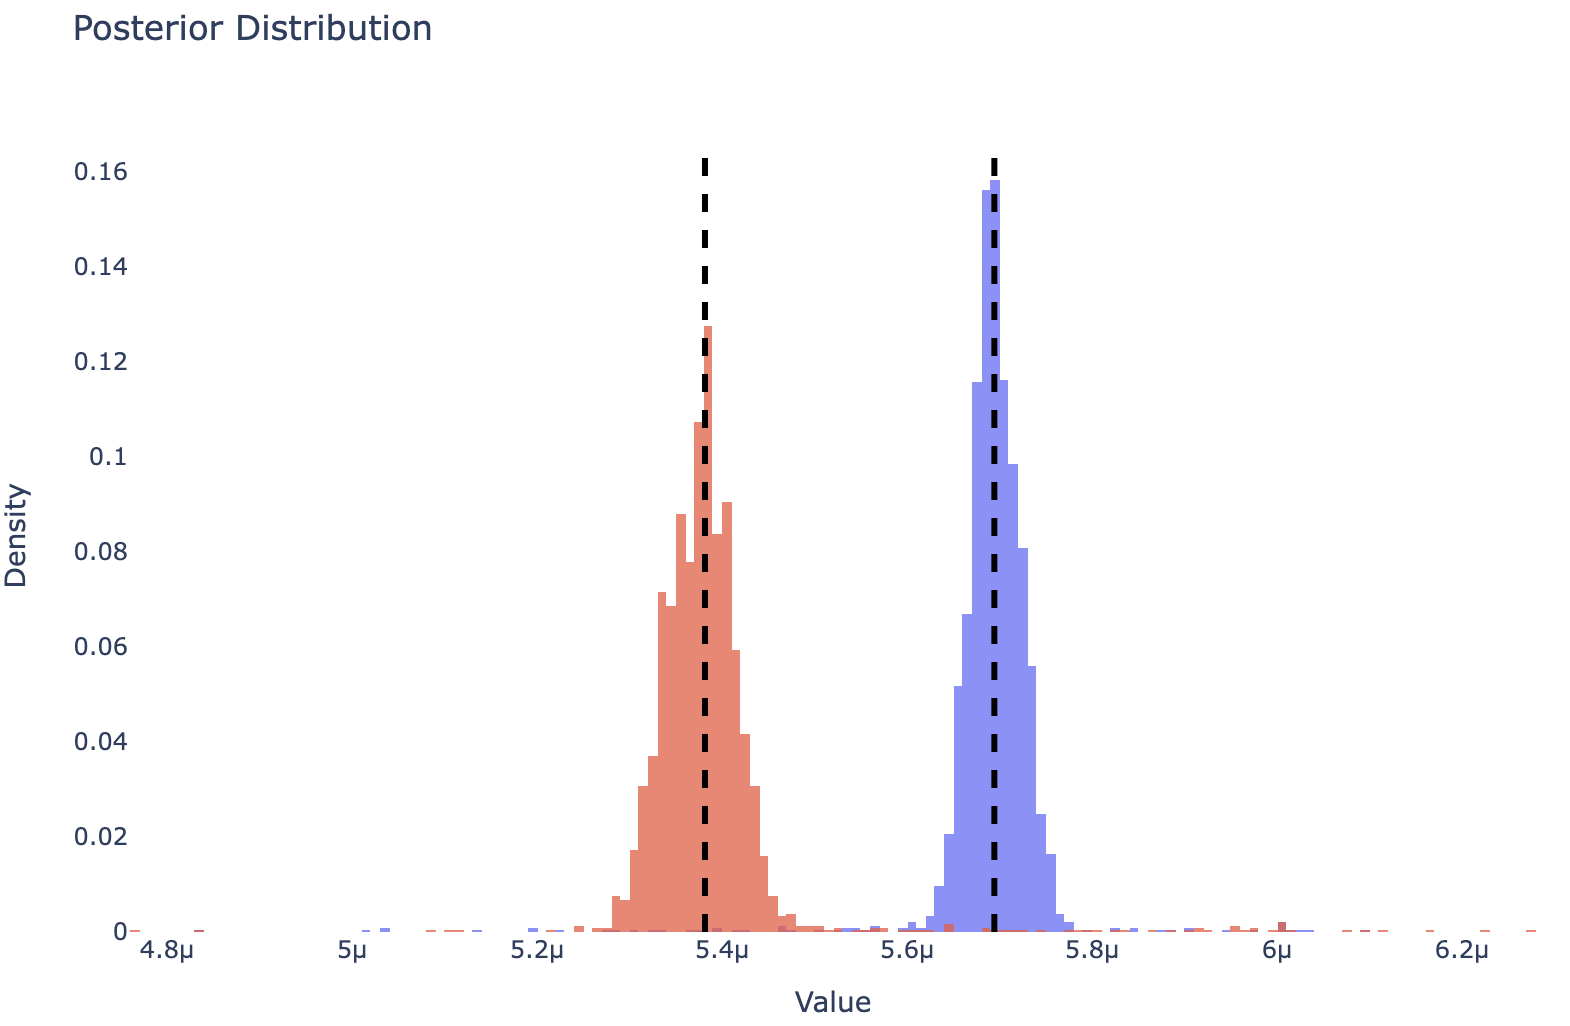
\includegraphics[width=0.455\textwidth]{Images/Highlights/SPMe posterior.png}
        % \caption{Caption}
        \label{fig:optimisersNew}
    \end{figure}
\end{frame}

\begin{frame}[fragile,t]{New in v24.9: Constrained optimisation}
    \vspace{-6mm}
    \issue{353} - Allows user defined nonlinear constraints

    \begin{figure}
        \centering
        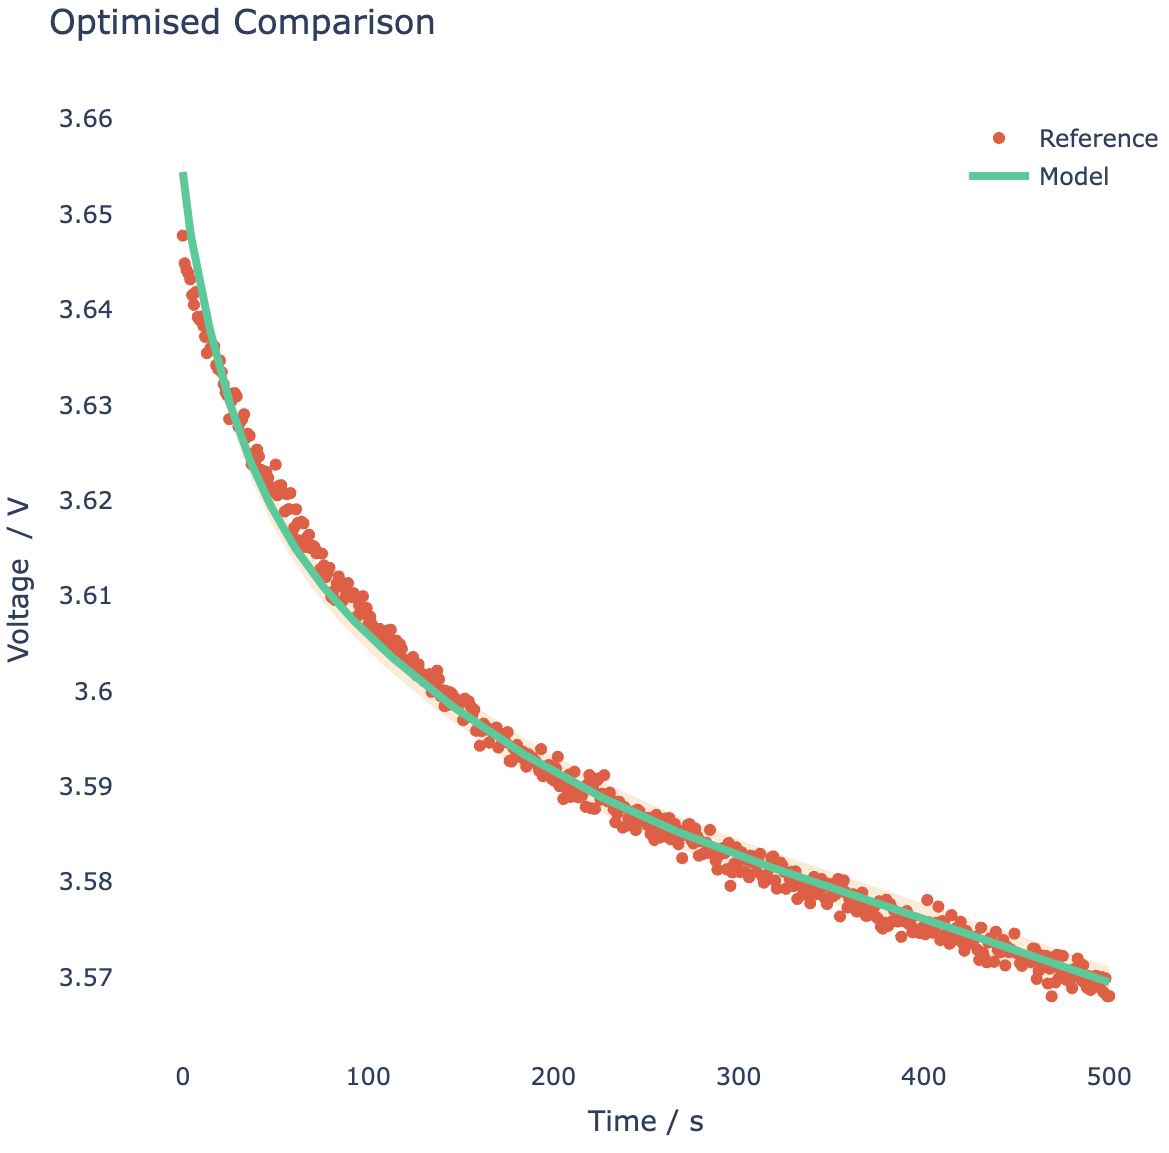
\includegraphics[width=0.37\textwidth]{Images/Highlights/trust-const-identification.png}
        \hspace{3em}
        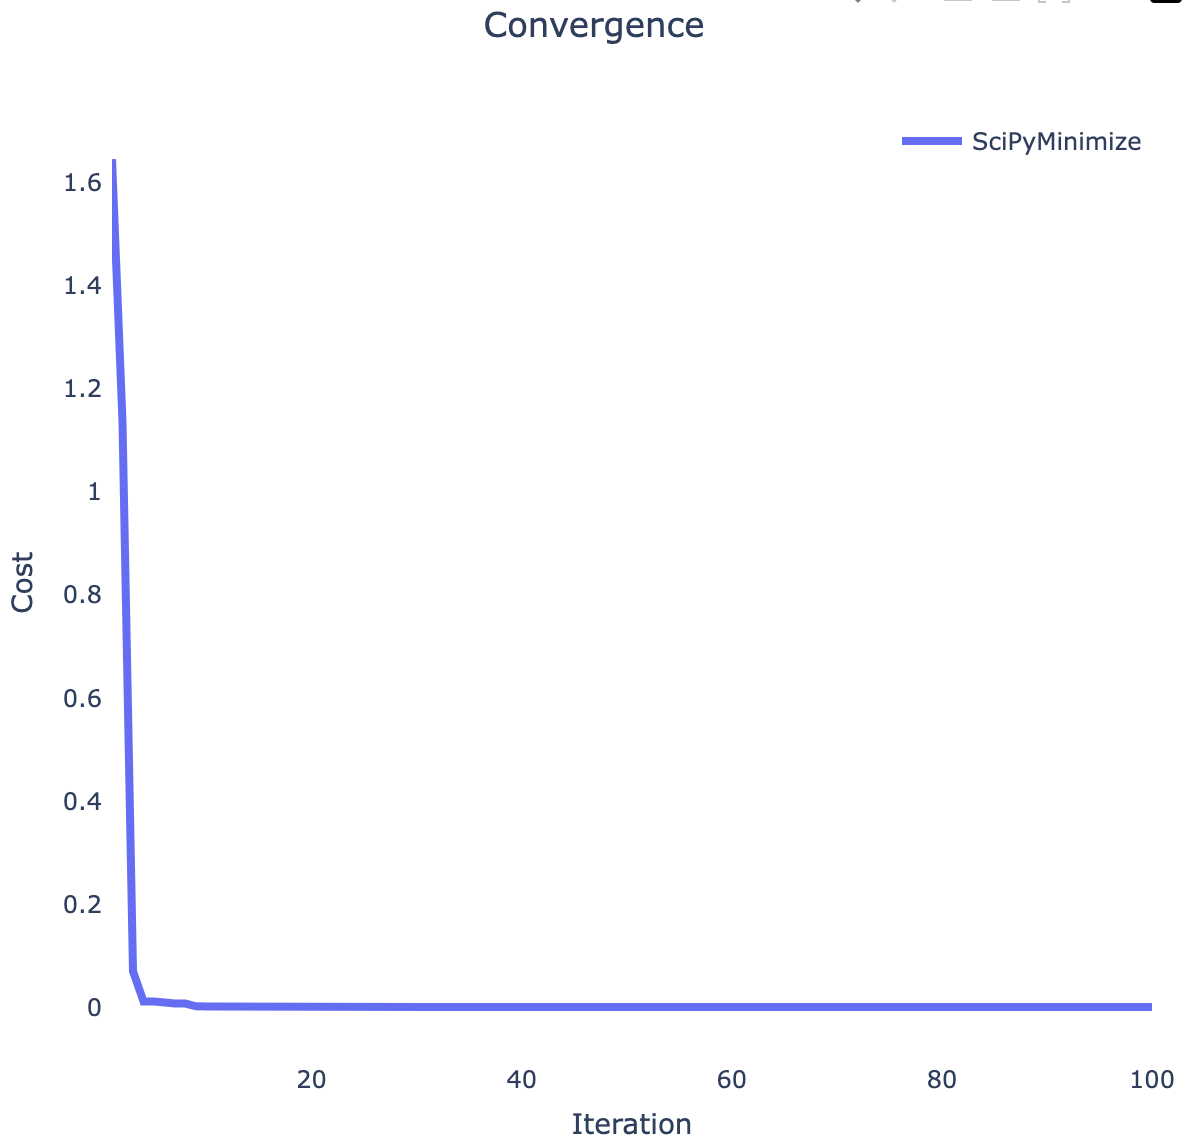
\includegraphics[width=0.37\textwidth]{Images/Highlights/trust-const-convergence.png}
        % \caption{Caption}
        \label{fig:WeppnerHuggins}
    \end{figure}
\end{frame}

\begin{frame}[fragile,t]{New in v24.9: Electrochemical impedance spectroscopy}
    \vspace{-6mm}
        \issue{405} - Adds EIS prediction methods

    \begin{figure}
        \centering
        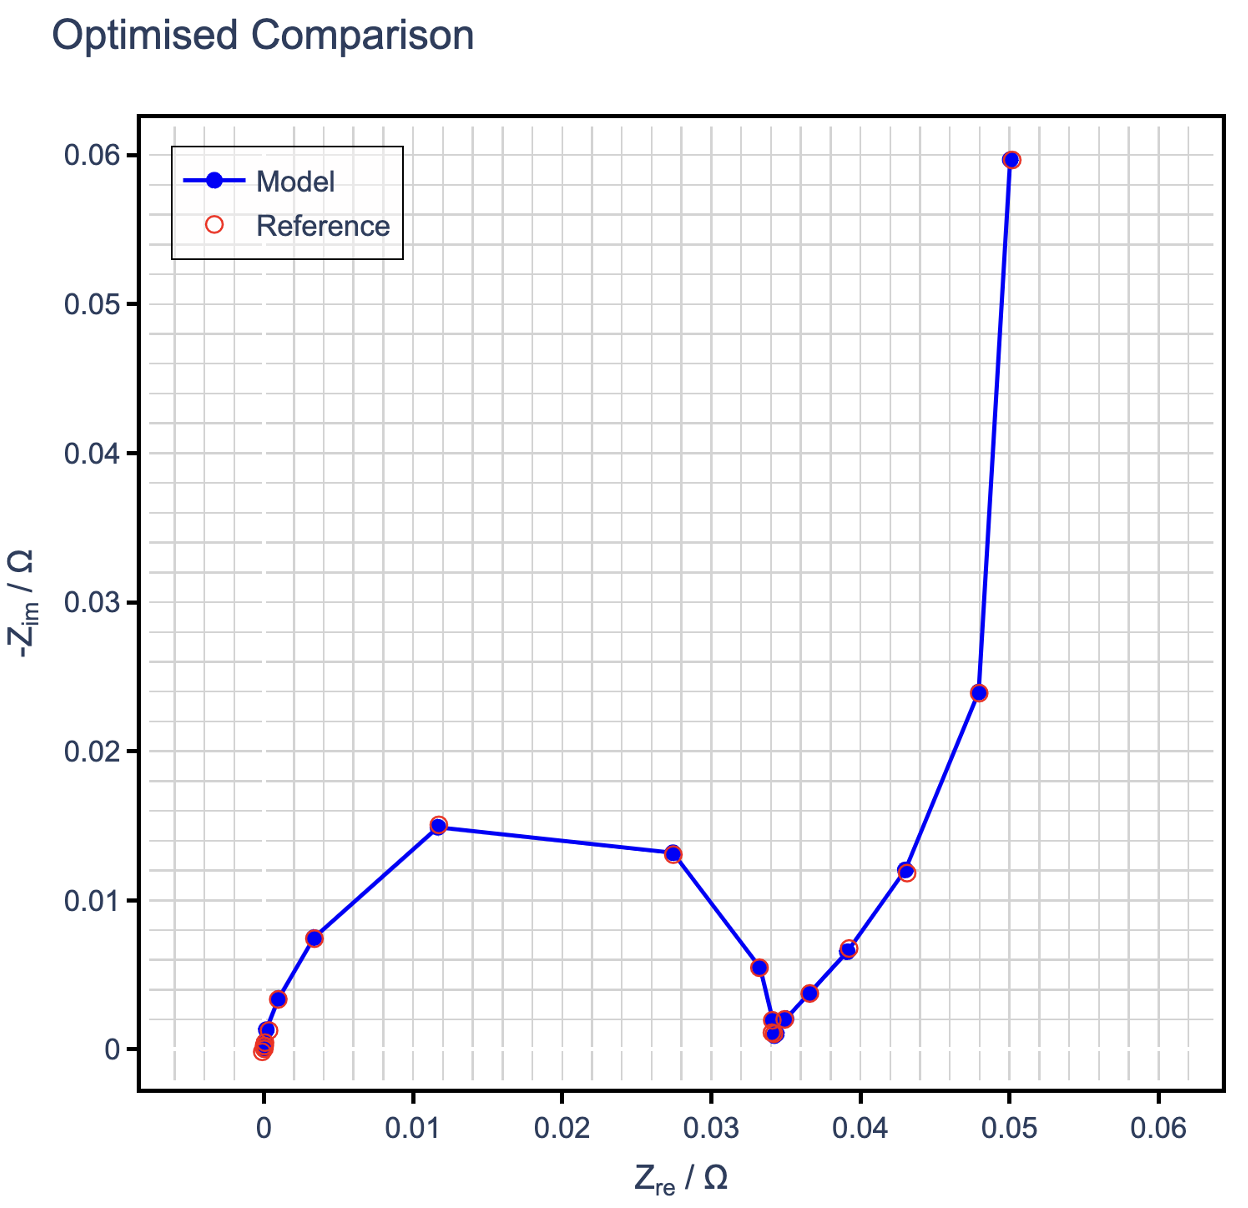
\includegraphics[width=0.35\textwidth]{Images/Highlights/nyquist-eis-identification.png}
        \hspace{3em}
        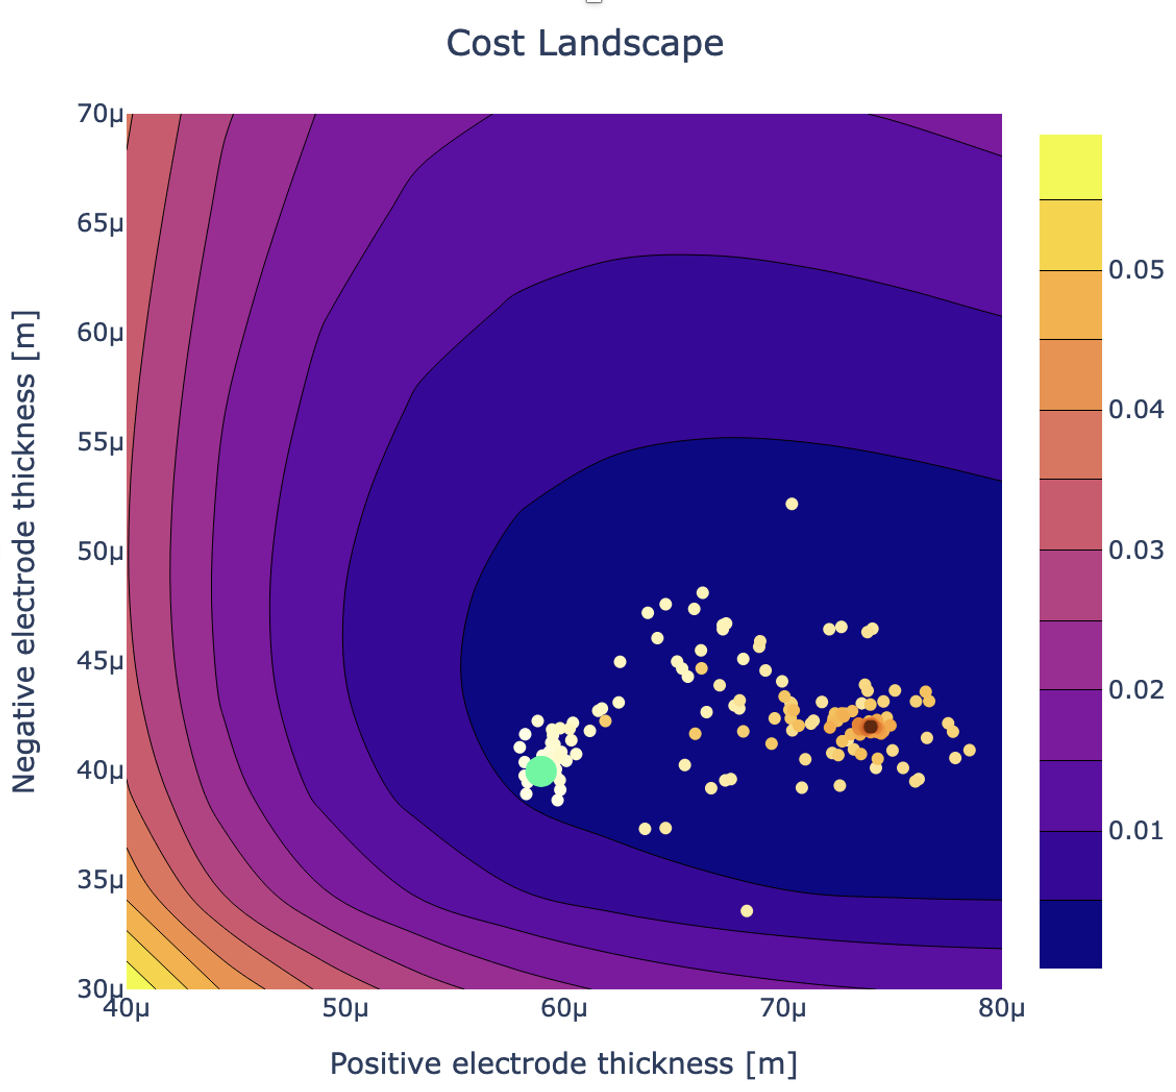
\includegraphics[width=0.37\textwidth]{Images/Highlights/eis-identification-landscape.png}
        % \caption{Caption}
        \label{fig:WeppnerHuggins}
    \end{figure}
\end{frame}

\begin{frame}[fragile,t]
\frametitle{New in 24.9: Weighted costs}
\vspace{-2em}
\begin{columns}
\begin{column}{0.5\textwidth}
\vspace{2em}
\begin{block}{Combine costs with weighting:}
\begin{lstlisting}[firstnumber=1, xleftmargin=10pt]
# Generate multiple cost functions and combine them
cost1 = pybop.GravimetricEnergyDensity(problem)
cost2 = pybop.VolumetricEnergyDensity(problem)
cost = pybop.WeightedCost(cost1, cost2, weights=[1, 1e-3])
\end{lstlisting}
\end{block}
\vspace{3.5em}
\end{column}
 % Right column with image
\begin{column}{0.5\textwidth}
%    \vspace{-1em}
    \begin{figure}
    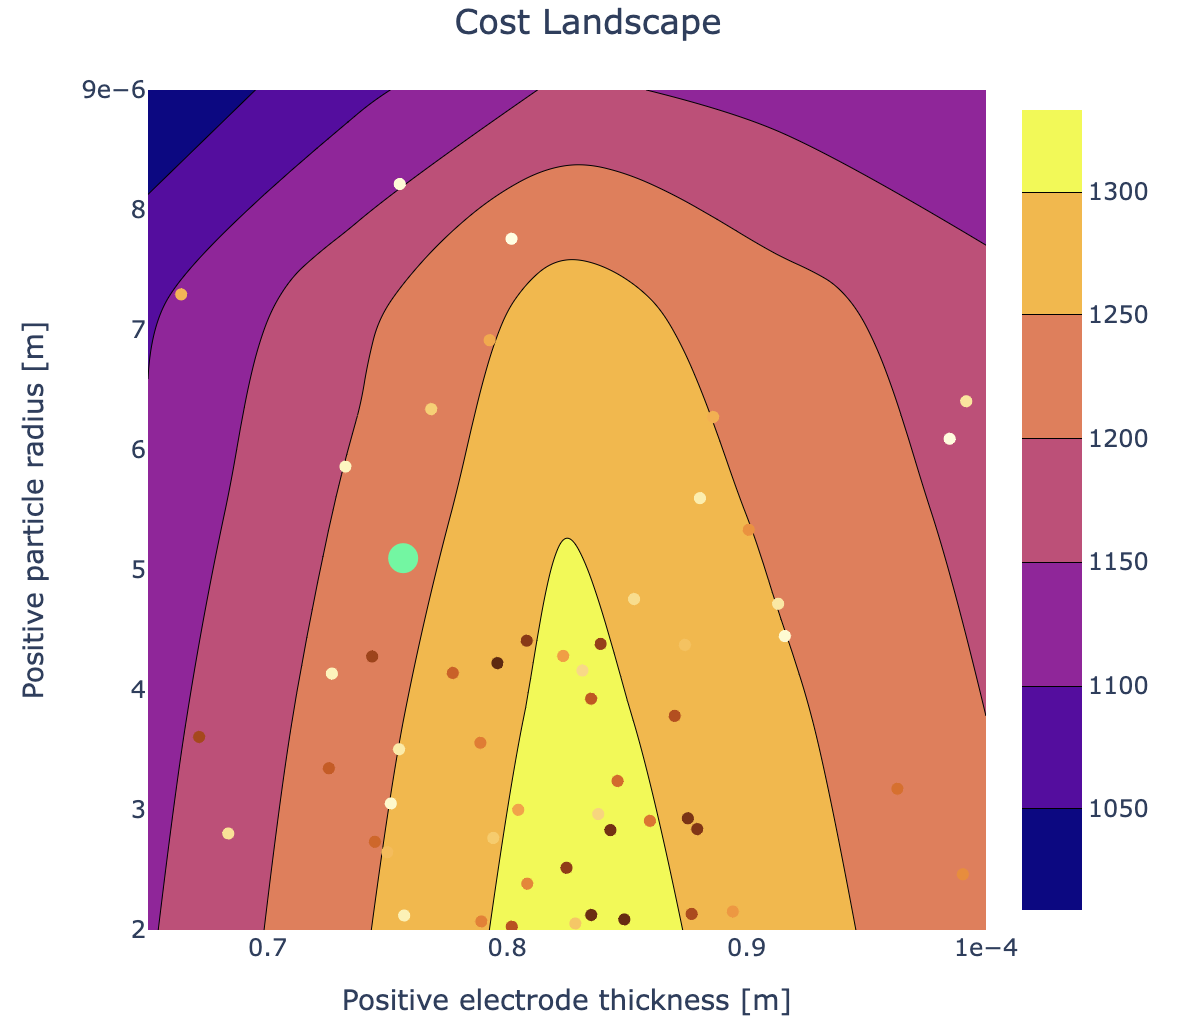
\includegraphics[width=0.94\textwidth]{Images/Highlights/weighted-design-landscape.png}
    \end{figure}
\end{column}
\end{columns}
\end{frame}

\begin{frame}[fragile,t]{New in v24.6: Experimental data fitting}
    \vspace{-6mm}
    \issue{241} - Adds experimental circuit model fitting notebook with LG M50 data from: \href{https://github.com/WDWidanage/Simscape-Battery-Library/tree/main/Examples/parameterEstimation_TECMD/Data}{https://github.com/WDWidanage/Simscape-Battery-Library/tree/main/Examples/parameterEstimation\_TECMD/Data}
    \begin{figure}
        \centering
        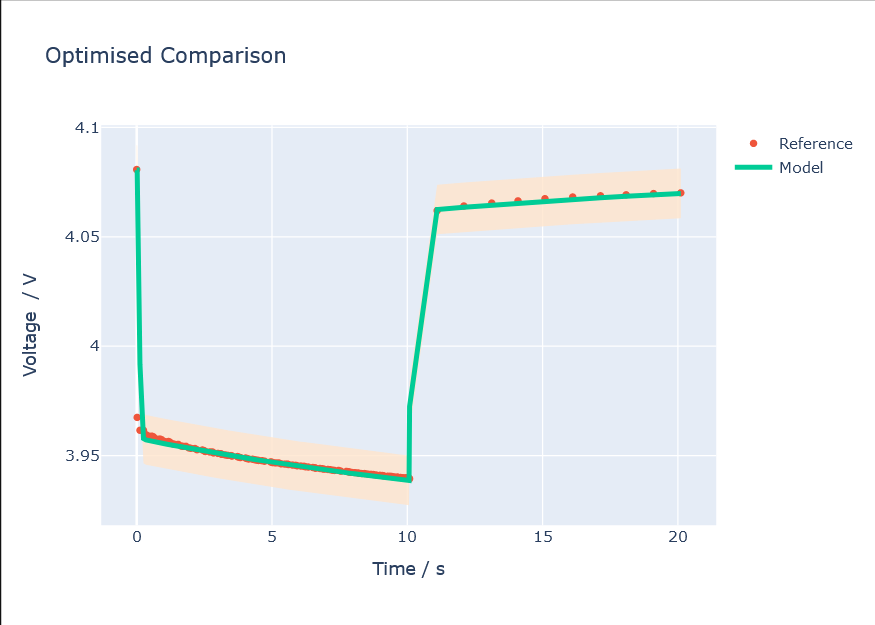
\includegraphics[height=0.3\textwidth]{Images/Highlights/LGM50_Fig1.png}
        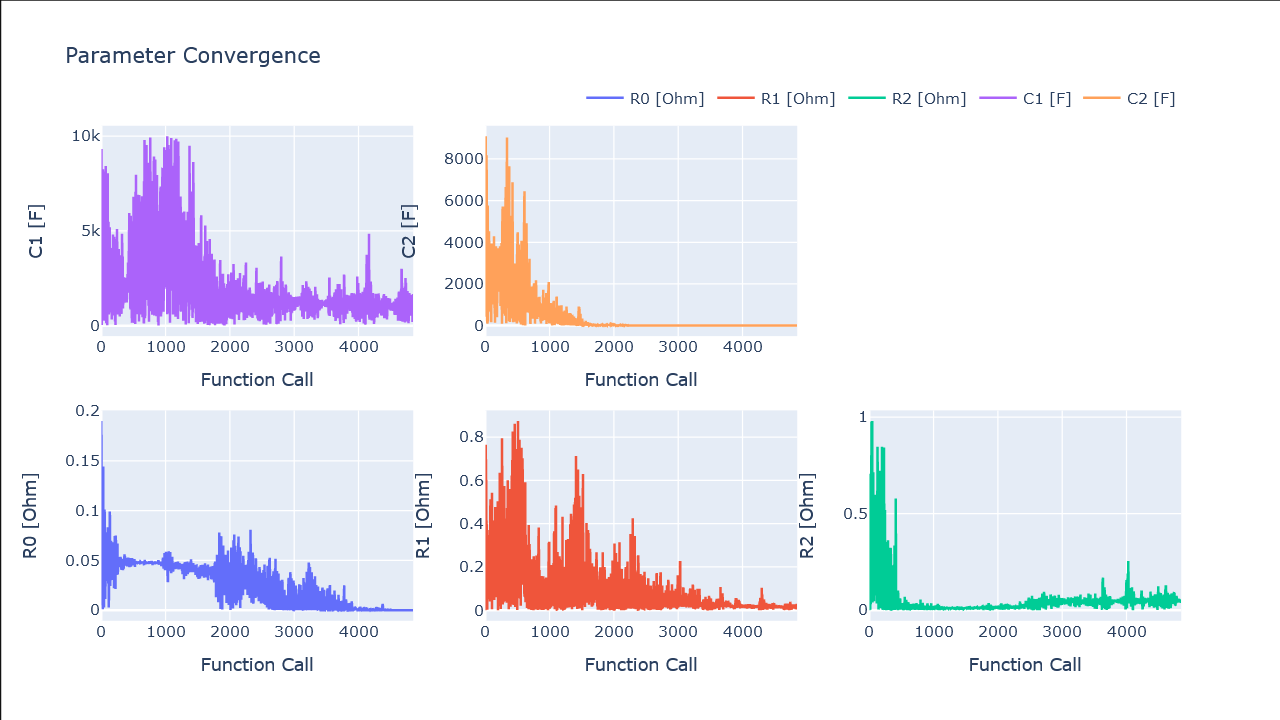
\includegraphics[height=0.3\textwidth]{Images/Highlights/LGM50_Fig2.png}
        \label{fig:LGM50}
    \end{figure}
\end{frame}

\begin{frame}{New in v24.6: Additional PyBaMM models}
    \vspace{-6mm}
    \issue{250} - Adds DFN, MPM, MSMR models and moves multiple construction variables to BaseEChem. Adds exception catch on simulate \& simulateS1.
    \begin{figure}
        \centering
        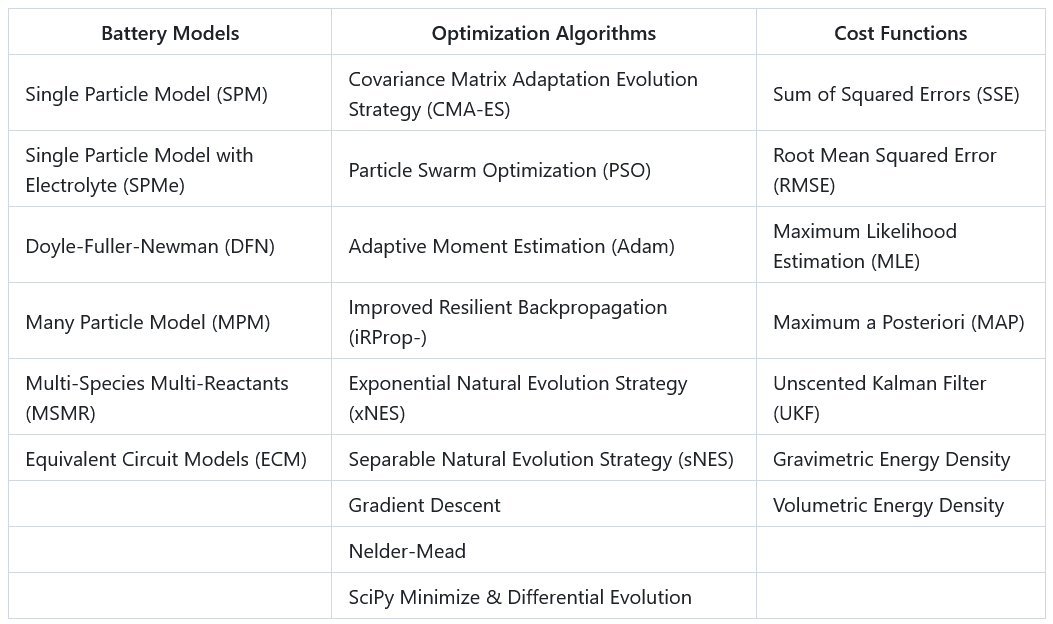
\includegraphics[height=0.35\textwidth]{Images/Diagrams/Supported_classes.png}
        \label{fig:supported_classes}
    \end{figure}
\end{frame}

\begin{frame}{New in v24.6: Maximum a Posteriori}
    \vspace{-6mm}
    \issue{275} - Adds Maximum a Posteriori (MAP) cost function with corresponding tests and example script.
    \begin{figure}
        \centering
        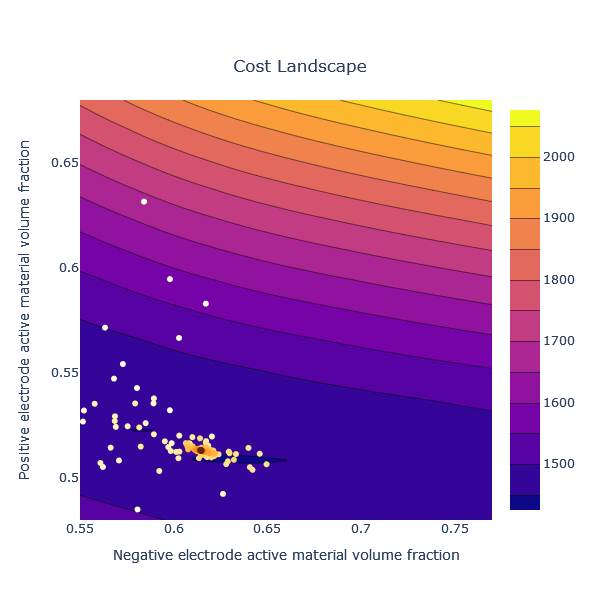
\includegraphics[height=0.35\textwidth]{Images/Highlights/MAP_param_convergence.png}
        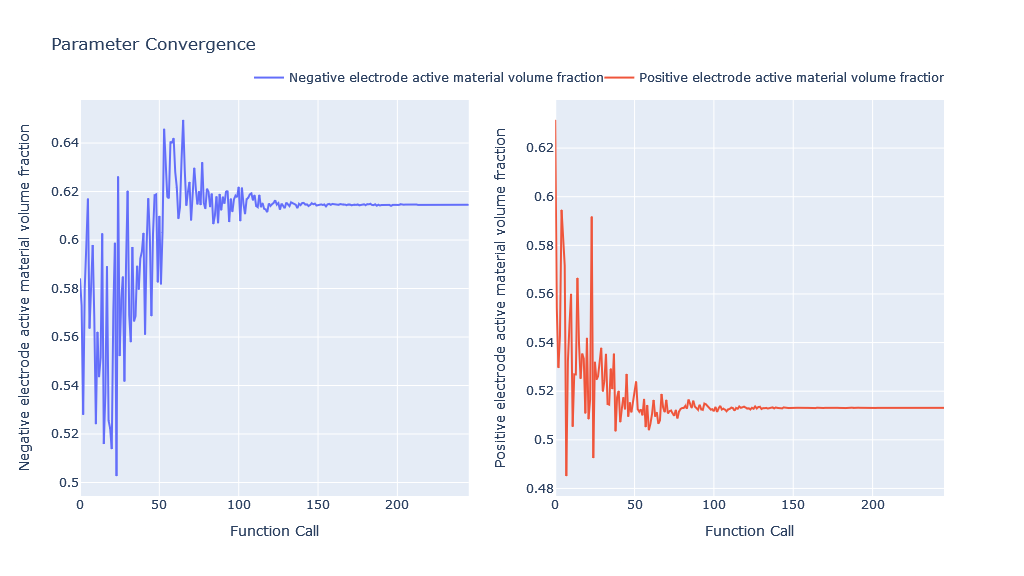
\includegraphics[height=0.35\textwidth]{Images/Highlights/MAP_cost_landscape.png}
        \label{fig:MAP_cost}
    \end{figure}
\end{frame}

\end{document}
